\documentclass[a4paper,11pt,oneside,openany]{jsbook}
%\documentclass[b5paper,10pt,oneside,openany]{jsbook}
%\documentclass[a4paper,10pt,oneside,openany]{jsbook}
%
\usepackage[dvipdfmx]{graphicx}
\usepackage{amsmath,amssymb}
\usepackage{bm}
\usepackage{graphicx}	
\usepackage{ascmac}
\usepackage{makeidx}
\usepackage{hyperref}
\usepackage{layout}
\usepackage{fancyhdr}
\usepackage{caption}
\usepackage{here}
\usepackage{url}
\usepackage{layout}

%\special{pdf:pagesize width 210mm height 297mm}

%
\providecommand{\tightlist}{\setlength{\itemsep}{0pt}\setlength{\parskip}{0pt}}
%
%図の前のコロンを削除%%%%%%%%
\makeatletter
\long\def\@makecaption#1#2{%
\vskip\abovecaptionskip
\iftdir\sbox\@tempboxa{#1\hskip1zw#2}%
\else\sbox\@tempboxa{#1 #2}%
\fi
\ifdim \wd\@tempboxa >\hsize
\iftdir #1\hskip1zw#2\relax\par
\else #1 #2\relax\par\fi
\else
\global \@minipagefalse
\hbox to\hsize{\hfil\box\@tempboxa\hfil}%
\fi
\vskip\belowcaptionskip}

% 図を強制的に指示した位置に入れる
\usepackage{here}
\renewcommand{\figurename}{Fig.}

%section書式設定%%%%%%%%
\renewcommand{\section}{\@startsection{section}{1}{\z@}%
   {0.5\Cvs \@plus0\Cvs \@minus 0.2\Cvs}% % section上部の空白量
   {0\Cvs \@plus0\Cvs \@minus 0.2\Cvs}%   % section下部の空白量
   {\reset@font\Large\bfseries}}          % フォント,フォントサイズを変更
\renewcommand{\subsection}{\@startsection{subsection}{2}{\z@}%
   {0.5\Cvs \@plus0\Cvs \@minus 0.2\Cvs}% 
   {0\Cvs \@plus0\Cvs \@minus 0.2\Cvs}%
   {\reset@font\large\bfseries}}
\renewcommand{\subsubsection}{\@startsection{subsubsection}{3}{\z@}%
   {0.5\Cvs \@plus0\Cvs \@minus 0.2\Cvs}% 
   {0\Cvs \@plus0\Cvs \@minus 0.2\Cvs}%
   {\reset@font\normalsize\bfseries}}
\makeatother
%%%%%%%%%%%%%%%%%%%%%%%%%%%%%
%
\makeindex
%レイアウト設定%%%%%%%%%%%%%%%%%%%%%%%%%%
\pagestyle{fancy}
\fancyhead{}
\fancyhead[LO]{\leftmark}
\fancyhead[RO]{\rightmark}
\renewcommand{\chaptermark}[1]{\markboth{第\ \thechapter\ 章~#1}{}}
\renewcommand{\sectionmark}[1]{\markright{\thesection #1}{}}

\cfoot{\thepage}

\renewcommand{\footrulewidth}{0.4pt}
%
\setlength{\textwidth}{389pt}
\setlength{\headwidth}{389pt}
\setlength{\textheight}{35.5\baselineskip}
\setlength{\footskip}{35pt}
\addtolength{\textheight}{\topskip}
\setlength{\voffset}{-0.65in}
%%%%%%%%%%%%%%%%%%%%%%%%%%%%%%%%%%%%%%%
\title{{\Huge \textbf{でしぷろノート Vol.06}}\\ {Matlab/SimulinkとArduinoでモータ回転数制御}}
\author{でし・ぷろんぷと\\ \texttt{http://deshi-prompt.github.io/}}
\date{Deshi Prompt 2018.8.10}
\begin{document}

\parindent = 0pt % 字下げしない

%------------------------------------------------------------------
% 表紙
\begin{titlepage}
    %\maketitle % 表紙の作成
    \begin{figure}[htbp]
        \centering
        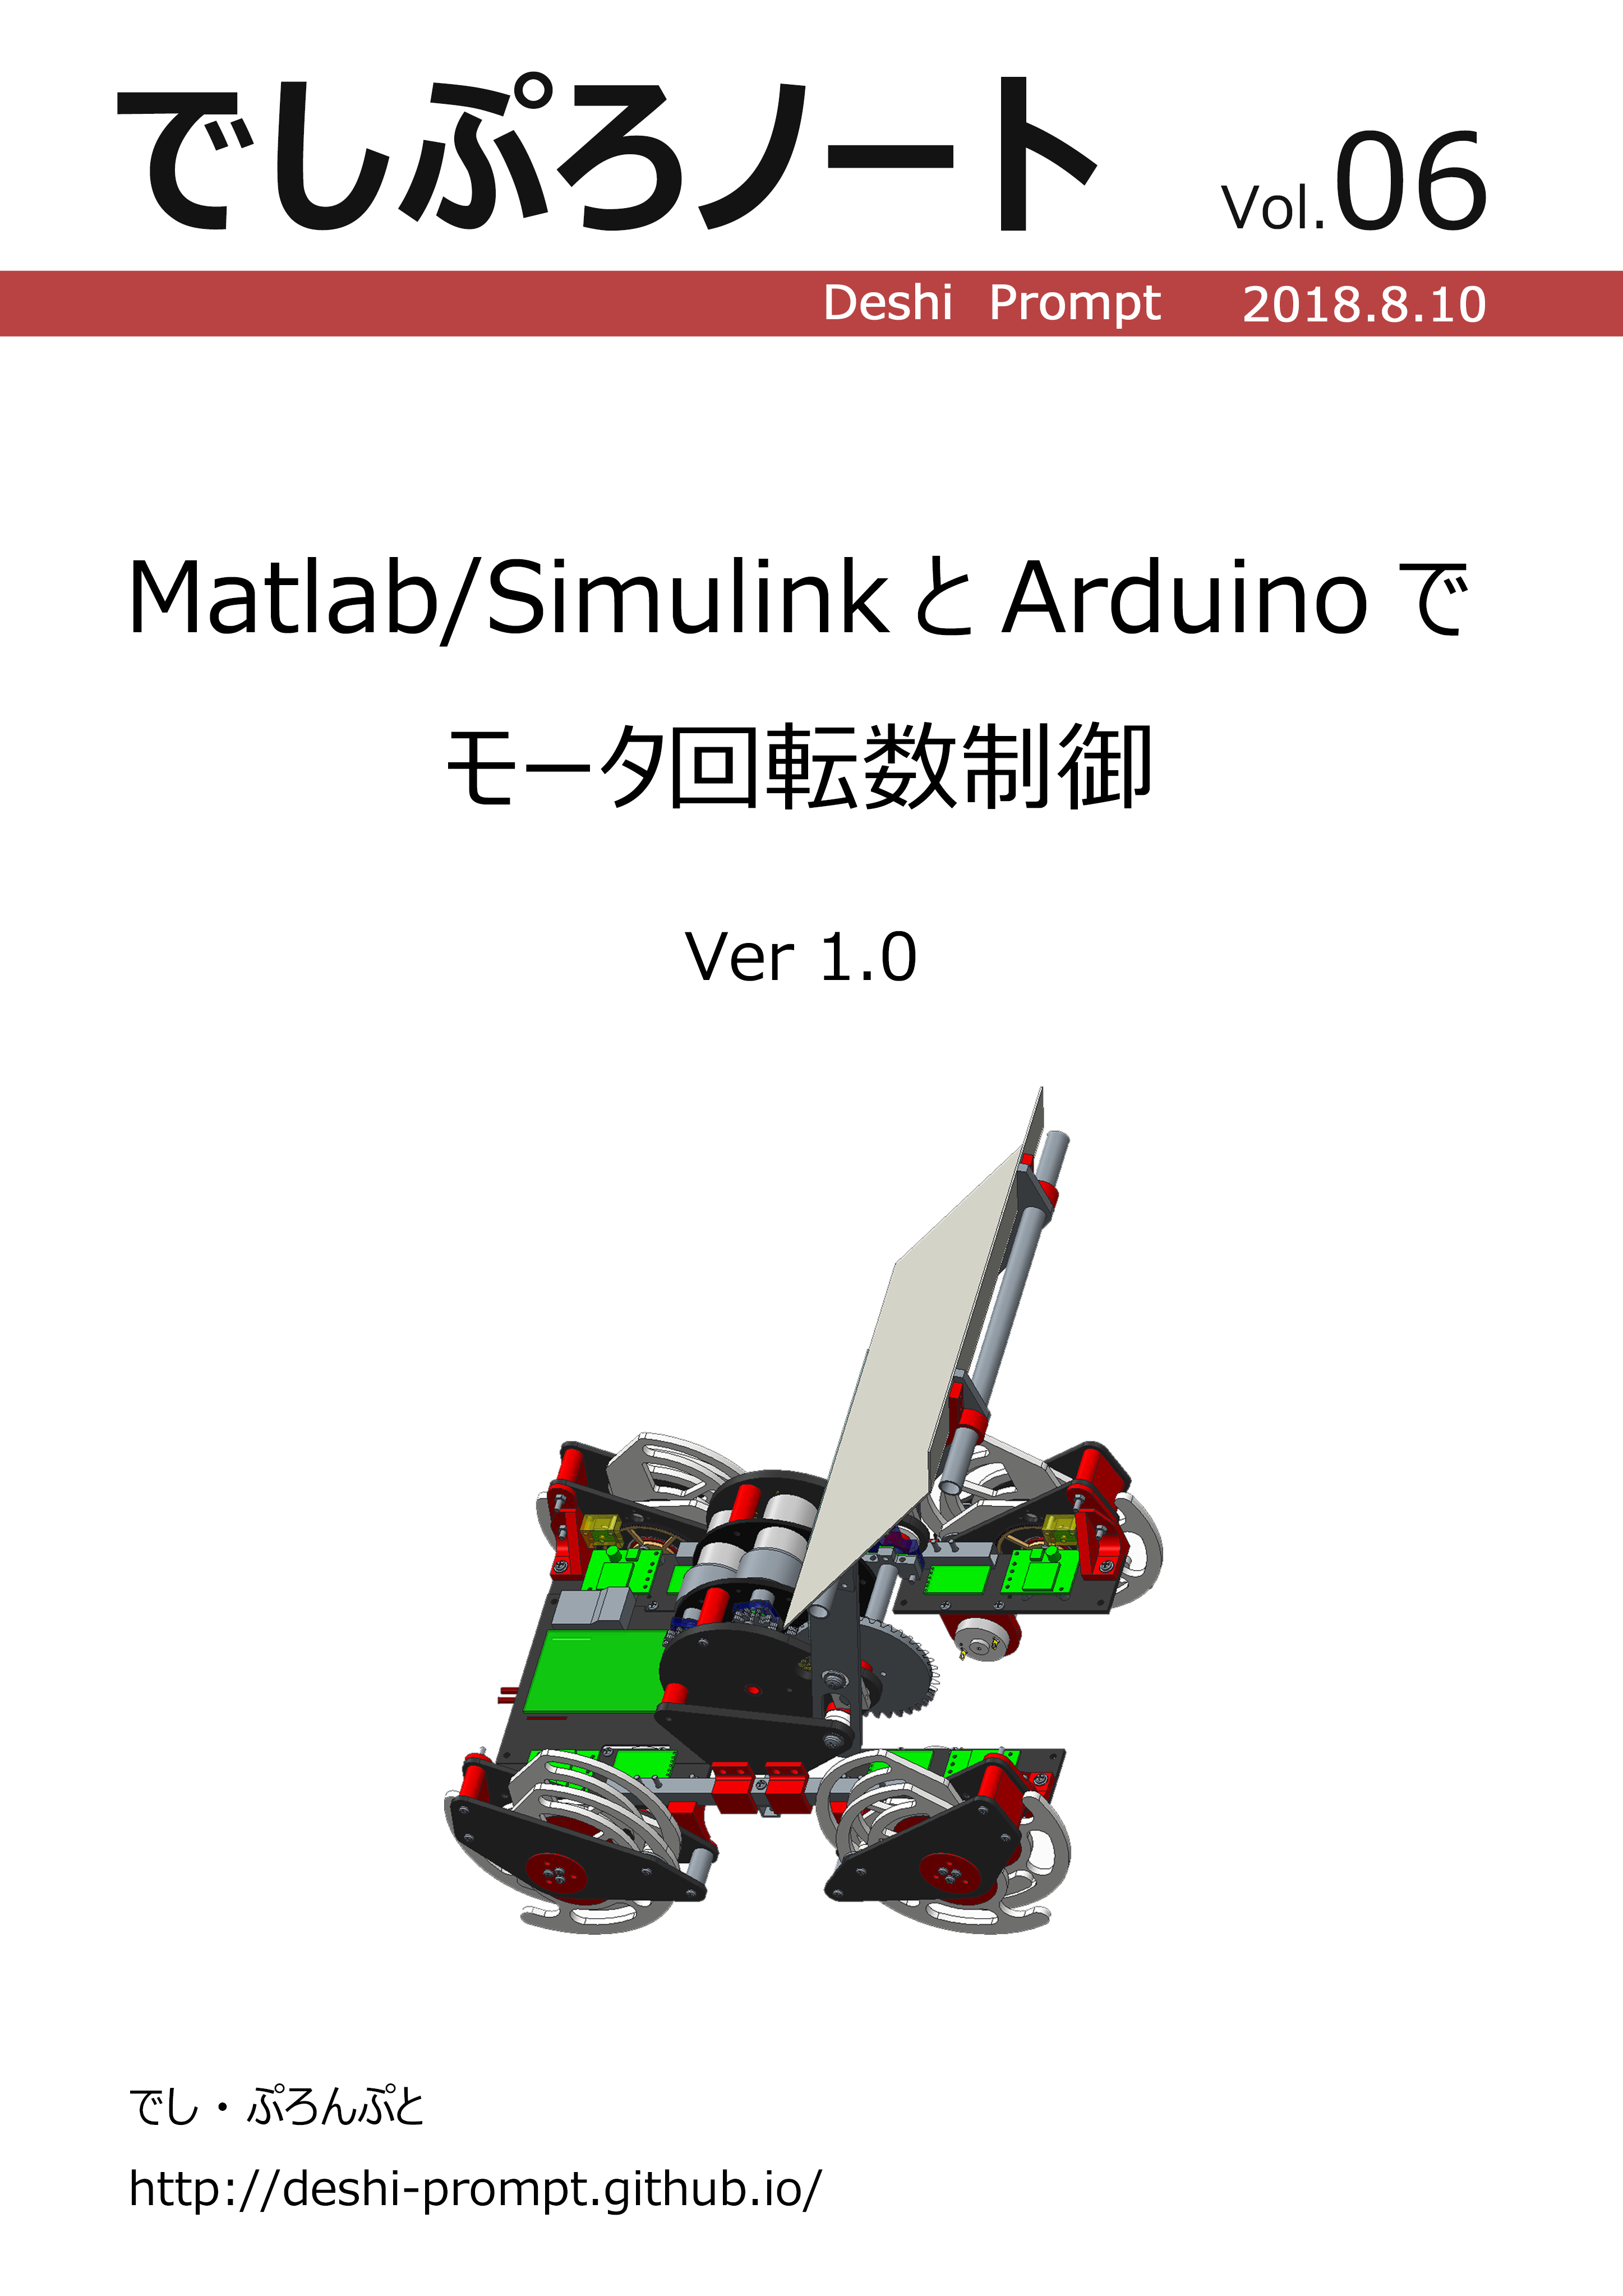
\includegraphics[width=350pt]{fig/title.png}
    \end{figure}
    \thispagestyle{empty}
\end{titlepage}

%------------------------------------------------------------------
%\thispagestyle{empty}
%\newpage 

%------------------------------------------------------------------
\frontmatter % 序文の開始
\setcounter{tocdepth}{1} %表示させる階層の深さを変更する 1:\sectionまで
\tableofcontents %目次作成
\thispagestyle{empty} 
%------------------------------------------------------------------
\mainmatter % 本文の開始


\setlength{\parskip}{1.5ex plus 0ex minus 0.2ex}

\chapter{はじめに}
\thispagestyle{fancy}
\section{本誌 概要}\label{ux6628ux4ecaux306ediyux4e8bux60c5}

本誌ではロボットハードウェア製作において、モータ回転数制御の実現方法を記載しています。
具体的な題材として、毎年川崎市で開催されている
「かわさきロボット競技大会」の機体製作を取り上げます。

\section{かわさきロボット競技大会の概要}\label{ux672cux8a8cux306eux4e2dux8eab}

かわさきロボット競技大会では、リング上で2台のロボットを戦わせます。
勝敗は審判の判定によって決定されます。
勝利条件の概略は下記の通りです。(大会HP\cite{kawasaki_public_HP}を参照)

\begin{itemize}
\tightlist
\item
  ラウンド内にリングの場外へ相手機体を押し出す
\item
  ラウンド内にリング上で相手機体をダウン(走行不可能な状態)させ、\\
  10カウントダウン状態をキープする
\end{itemize}

製作する機体の概略は下記の通りです。
詳細はかわさきロボット競技大会公式サイト\cite{kawasaki_public_HP}に記載されています。
参考までに筆者が過去に製作した機体はFig.\ref{fig101}です。

\begin{itemize}
\tightlist
\item
  サイズ制限:全幅250mm × 全長350mm × 高さ700mm(スタート時)
\item
  重量制限:3300g以内
\item
  操縦は、競技大会の実行委員会が規定するプロポを用いること
\item
  ロボットには、それぞれ1セット以上の脚機構、アーム機構が搭載されていること
\item
  ロボットは走行用の脚部と相手機体への攻撃用のアーム部を有する
\end{itemize}

\begin{figure}[htbp]
\centering
\includegraphics[width=380pt]{fig/fig101.eps}
\caption{筆者のかわさきロボット出場機体}
\label{fig101}
\end{figure}


\section{ロボット操縦の課題}\label{ux672cux8a8cux306eux5bfeux8c61ux8005}

製作したロボットは例えば左右の脚ユニットの負荷ばらつき、モータの性能ばらつき等で
同じ操作量を入れてもFig.\ref{fig102}のように思った方向に進まない場合があります。

\begin{figure}[htbp]
\centering
\includegraphics[width=280pt]{fig/fig102.eps}
\caption{ロボットの動き}
\label{fig102}
\end{figure}

そこで、Fig.\ref{fig103}のようにモータの回転数に対して
フィードバック制御を入れ、左右の回転数差を無くします。

\begin{figure}[htbp]
\centering
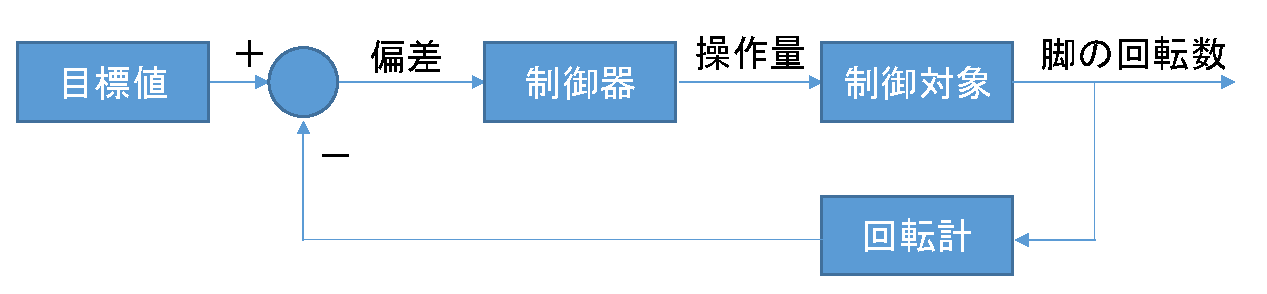
\includegraphics[width=280pt]{fig/fig103.eps}
\caption{フィードバック制御}
\label{fig103}
\end{figure}

ロボット制御システムのハードウェア構成例として、Fig.\ref{fig104}の通りです。
今回、制御プログラムをMatlab/Simulink上で構築してArduinoで動かすことを目指します。

\begin{figure}[htbp]
\centering
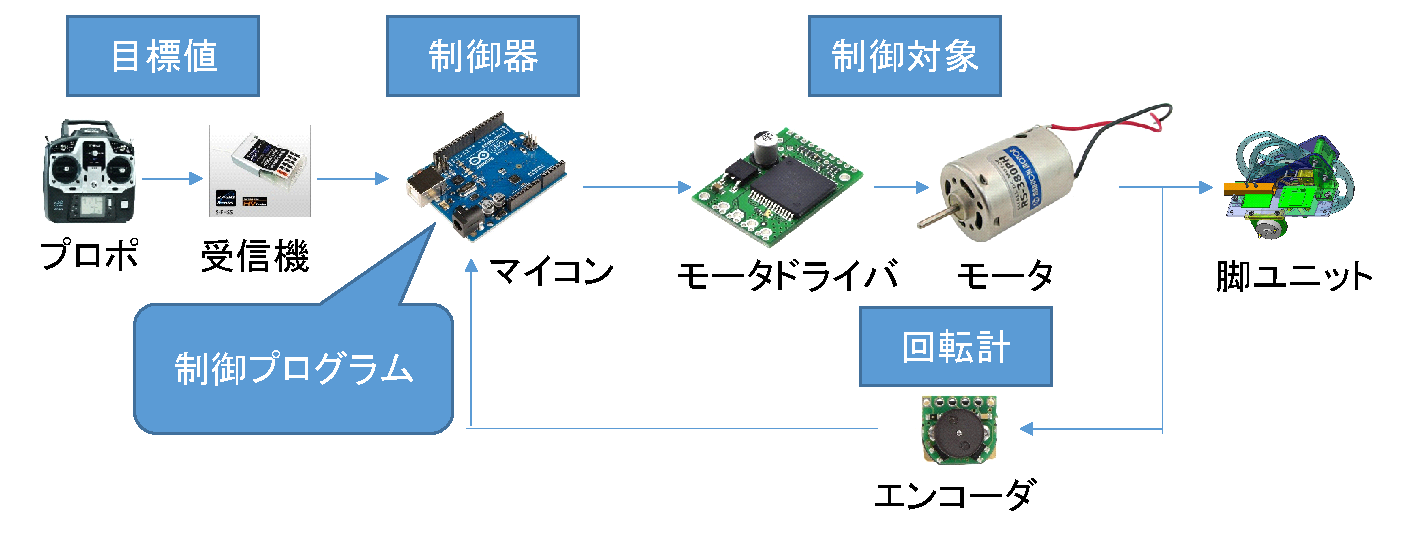
\includegraphics[width=250pt]{fig/fig104.eps}
\caption{ロボット制御システムのハードウェア構成例}
\label{fig104}
\end{figure}


\section{Matlab/Simulink開発環境構築}\label{ux5927ux578bux90e8ux54c1ux306eux4f5cux6210ux65b9ux6cd5}

本書執筆時の動作環境を下記に示します。

\begin{itemize}
  \tightlist
  \item
   OS:Windows 10 64bit
  \item
   Matlab/Simulink:R2018a
   \item
   Arduino:Mega 2560 R3 または Uno R3
\end{itemize}

\subsection{Matlab/Simulinkのインストール}\label{ux6a5fux4f54}

個人ライセンス製品の MATLAB Home \cite{MathWorks_HP} を使います。\\
2018年8月時では、MATLAB本体は¥16,500、Simulinkは¥4,990 です。


\subsection{Simulink での Arduino 動作環境をインストール}\label{ux6a5fux4f55}

Matlab起動時のメニューにある "アドオン" ⇒ "ハードウエアサポートパッケージの入手" を
クリックします。
アドオン エクスプローラーで、
Simulink Support Package for Arduino Hardware (Fig.\ref{fig105}) を
選択してインストールします。

\begin{figure}[htbp]
  \centering
  \includegraphics[width=130pt]{fig/fig105.eps}
  \caption{アドオン エクスプローラー}
  \label{fig105}
  \end{figure}


%\clearpage  
\subsection{C言語コンパイラのインストール}\label{ux5bfeux7b56ux6848}

第3章に記載している S-Function Builder ブロックを使用するためにはC言語コンパイラが必要です。

C言語コンパイラ有無の確認は、Matlab コマンドウインドウに下記を入力して実行します。

mex -setup

C言語コンパイラがすでにインストールされていればFig.\ref{fig107}のような表示が出ます。

C言語コンパイラがインストールされていなければ、インストールが必要です。

今回、C言語コンパイラとして、フリーで入手できる Microsoft Windows SDK 7.1 を使用します。

ただし、Microsoft Windows SDK 7.1 は
最新OSだと通常のやり方ではインストールできません\cite{Win_SDK1} \cite{Win_SDK2}。

Microsoft Windows SDK 7.1 インストール手順のポイントを次に示します。


\subsubsection{i. Visual C++ 2010のランタイムをアンインストールする}\label{sec:section1.4.1-1}

下記プログラムが既にインストールされていると、SDKのインストールに失敗するので\\
"アプリと機能" からアンインストールします。

\begin{itemize}
  \tightlist
  \item
  Microsoft Visual C++ 2010 x86 Redistributable
  \item
  Microsoft Visual C++ 2010 x64 Redistributable
  \end{itemize}


\clearpage
\subsubsection{ii. winsdk-web.exeのインストール}\label{sec:section1.4.1-2}

下記ホームページからインストーラをダウンロードして、インストールします。

\url{http://www.microsoft.com/en-us/download/details.aspx?id=8279}

インストール設定画面において、
Microsoft Visual C++2010 のチェックを外してください (Fig.\ref{fig106}) 。

\begin{figure}[htbp]
  \centering
  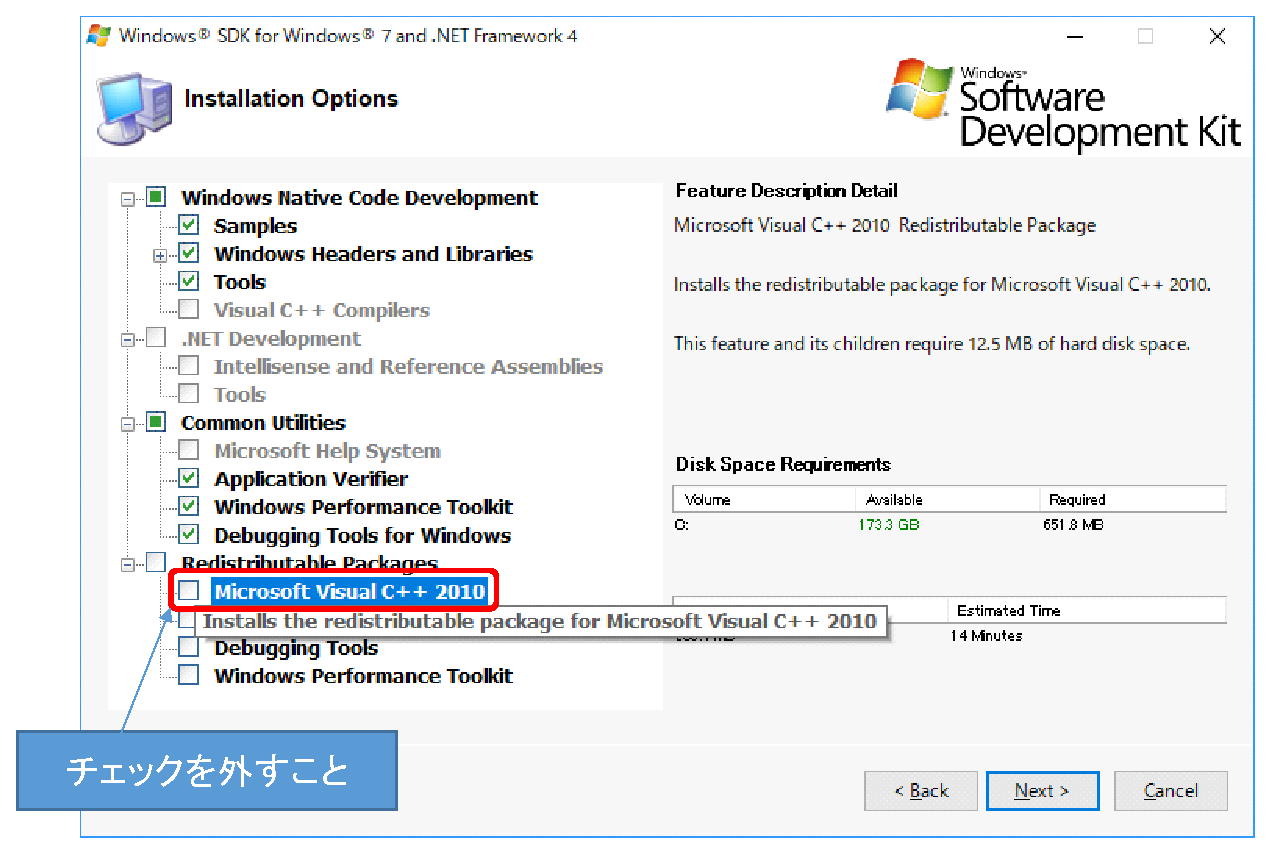
\includegraphics[width=200pt]{fig/fig106.eps}
  \caption{SDK 7.1 インストール設定画面}
  \label{fig106}
  \end{figure}


\subsubsection{iii. VC-Compiler-KB2519277.exeのインストール}\label{sec:section1.4.1-3}

下記ホームページからインストーラをダウンロードして、インストールします。

\url{http://www.microsoft.com/en-us/download/details.aspx?id=4422}

\subsubsection{iv. 正しくインストールされたか確認}\label{sec:section1.4.1-4}

Matlab コマンドウインドウに mex -setup を実行して、
Fig.\ref{fig107}の表示がでればインストールは完了です。

\begin{figure}[htbp]
  \centering
  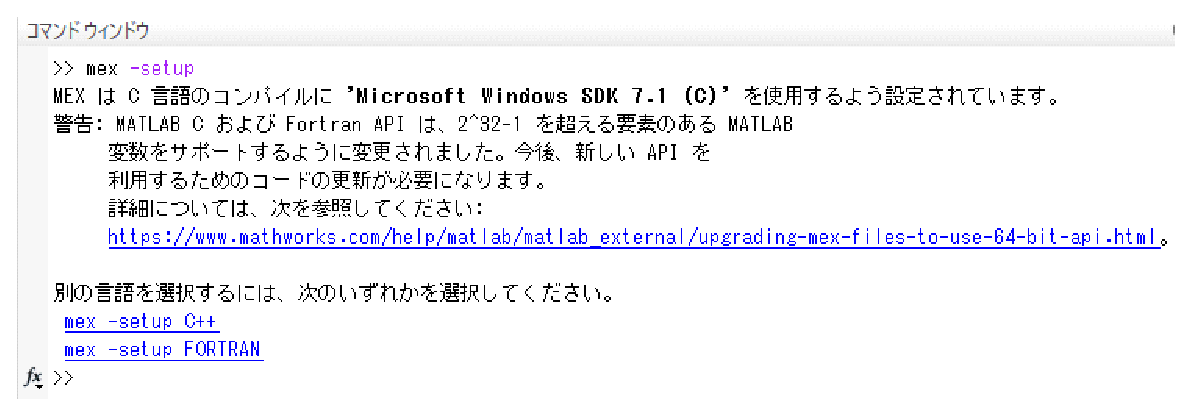
\includegraphics[width=300pt]{fig/fig107.eps}
  \caption{Matlab コマンドウインドウ}
  \label{fig107}
  \end{figure}

\chapter{Matlab/SimulinkとArduinoでモータを動かそう}
\thispagestyle{fancy}
\section{ハード構成}\label{dux30d7ux30eaux30f3ux30bfux306eux57faux672cux539fux7406}

本章では、かわさきロボット大会指定の380モータではなく、
手っ取り早くモータ制御を実現するために、市販されているハード(Fig.\ref{fig201})で構成しました。
全てのハードは通販サイト、例えばスイッチサイエンス \cite{switch-science_HP} から購入できます。
既存のハードでモータ制御を学んだのちに、ロボット本体へ適用します。

\begin{itemize}
    \tightlist
    \item
    マイコン:Arduino Mega 2560 R3
    \item
    モータドライバ:VNH5019搭載モータードライバ (POLOLU-1451)
    \item
    モータ:75:1 シャフト付き超小型メタルギアドモーター HP (POLOLU-2215)
    \end{itemize}

\begin{figure}[htbp]
\centering
\includegraphics[width=300pt]{fig/fig201.eps}
\caption{ハード構成}
\label{fig201}
\end{figure}


\section{回路図}\label{ux71b1ux6eb6ux89e3ux7a4dux5c64ux6cd5fdm}

回路図は、Fig.\ref{fig202}の通りです。
Arduino Mega 2560 のピン5~7を使用してモータドライバを動かします。
モータドライバ VNH5019 の詳細は、
Pololu HP \cite{pololu_HP_driver} に記載されています。

\begin{figure}[htbp]
\centering
\includegraphics[width=350pt]{fig/fig202.eps}
\caption{回路図}
\label{fig202}
\end{figure}


\section{Simulinkモデル}\label{ux71b1ux6eb6ux89e3ux7a4dux5c64ux65b9ux6cd5ux306eux7279ux5fb4}

Simulinkモデルは、Fig.\ref{fig203}の通りです。
ArduinoをSimulink上で実行できるように、シミュレーションモードを "エクスターナル" に、
シミュレーション終了時間を "inf" に変更します。

コンフィギュレーション パラメーターを開き、
ハードウェア実行 ⇒ ハードウェア ボードを "Arduino Mega 2560" にします(Fig.\ref{fig204})。

指令値をモータドライバの制御信号に変換するために、MATLAB Function ブロックを使用します。
ブロックの中身は、Fig.\ref{fig205}の通りです。
プロポからのラジコン信号入力を想定して、1500usec付近でモータ停止、
1150~1850usecの間で速度変更する仕様としてます。

\begin{figure}[htbp]
\centering
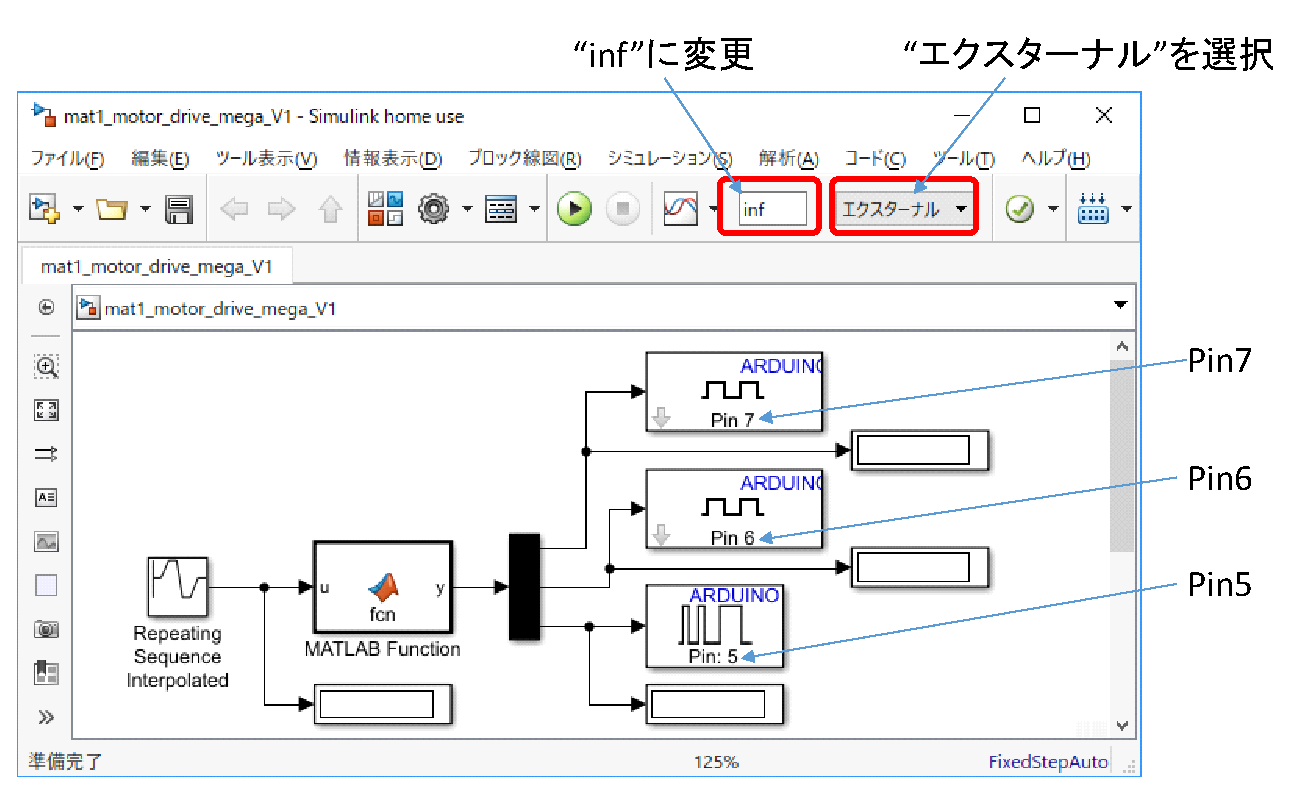
\includegraphics[width=350pt]{fig/fig203.eps}
\caption{Simulinkモデル}
\label{fig203}
\end{figure}

\begin{figure}[htbp]
\centering
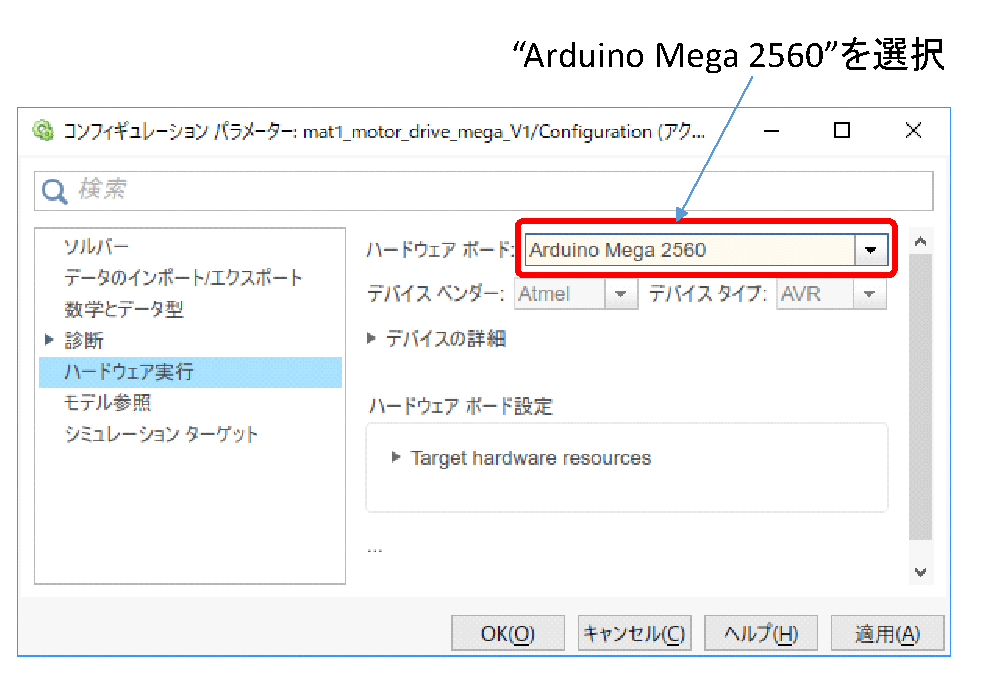
\includegraphics[width=300pt]{fig/fig204.eps}
\caption{コンフィギュレーション パラメーター}
\label{fig204}
\end{figure}

\begin{figure}[htbp]
\centering
\includegraphics[width=380pt]{fig/fig205.eps}
\caption{MATLAB Function ブロックの中身}
\label{fig205}
\end{figure}


\clearpage
\section{実行}\label{dux30d7ux30eaux30f3ux30bfux306eux57faux672cux7684ux306aux69cbux9020}

Fig.\ref{fig206}に示すボタンをクリックすることでプログラムを実行できます。

Simulinkと連動して動作させる場合は "実行" をクリックします。
ビルドに成功して動作し始めると、Display ブロックに出力値がリアルタイムに表示されます。
また、入力値として使用した Repeating Sequence Interpolated ブロックをダブルクリックし、
パラメータを変更することで、実行しながらもパラメータ変更の挙動が確認できます。

Simulinkと連動させず、Arduinoをスタンドアロンで動かす場合は "ハードウェアに展開" をクリックします。
一度書き込めば、Simulinkと接続しなくてもプログラムが動くようになります。

\begin{figure}[htbp]
\centering
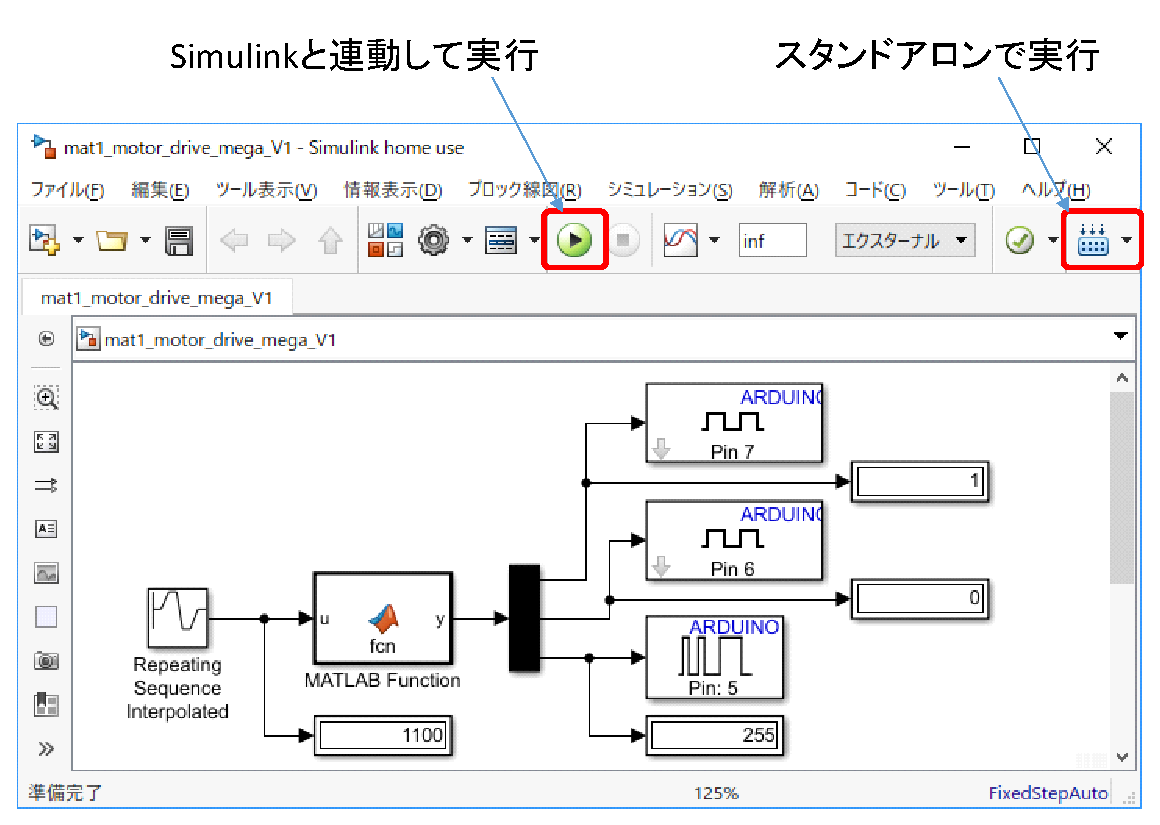
\includegraphics[width=350pt]{fig/fig206.eps}
\caption{Matlab/Simulinkモデルの実行}
\label{fig206}
\end{figure}


\chapter{Matlab/SimulinkとArduinoでモータ回転数を計測しよう}
\thispagestyle{fancy}
\section{ハード構成}\label{ux30edux30dcux30c3ux30c8ux7af6ux6280ux5927ux4f1aux306eux6982ux8981}

ハード構成はFig.\ref{fig301}の通りです。
Fig.\ref{fig201}よりエンコーダを追加することで、モータの回転数を取得します。

\begin{itemize}
    \tightlist
    \item
    マイコン:Arduino Mega 2560 R3
    \item
    モータドライバ:VNH5019搭載モータードライバ (POLOLU-1451)
    \item
    モータ:75:1 シャフト付き超小型メタルギアドモーター HP (POLOLU-2215)
    \item
    エンコーダ:シャフト付き超小型メタルギアドモーター用磁気式エンコーダ (POLOLU-3081)
    \end{itemize}

\begin{figure}[htbp]
\centering
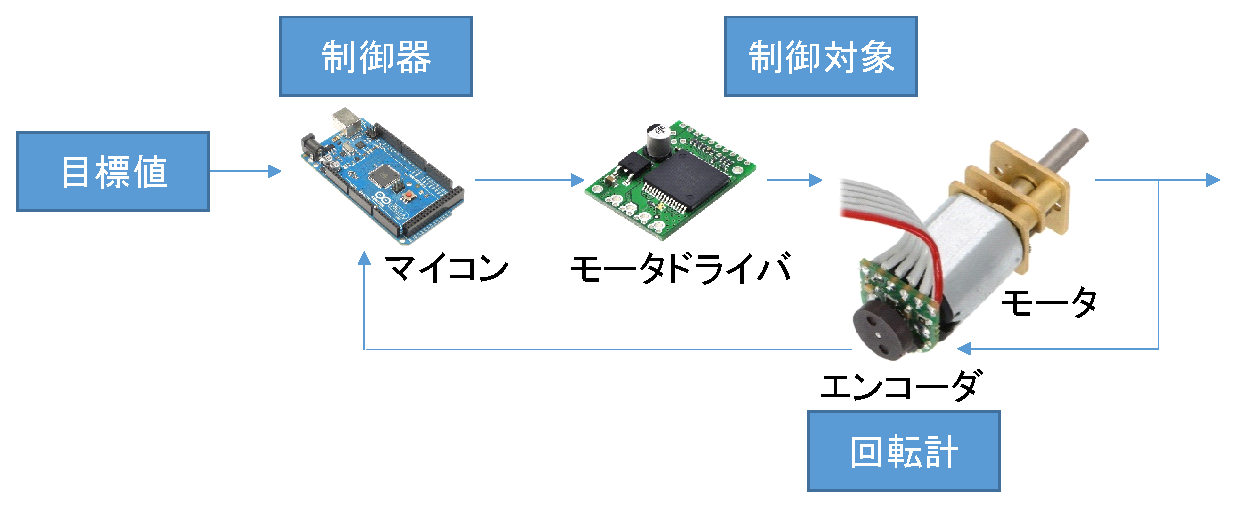
\includegraphics[width=300pt]{fig/fig301.eps}
\caption{ハード構成}
\label{fig301}
\end{figure}


\section{回路図}\label{ux69cbux60f3ux8a2dux8a08}

回路図はFig.\ref{fig302}の通りです。
Arduino Mega 2560 のピン2~3を使用してエンコーダ信号を読み取ります。
エンコーダの詳細は、Pololu HP \cite{pololu_HP_encoder} に記載されています。

\begin{figure}[htbp]
\centering
\includegraphics[width=380pt]{fig/fig302.eps}
\caption{回路図}
\label{fig302}
\end{figure}


\section{Simulinkモデル}\label{ux5168ux4f53ux69cbux6210}

Simulinkモデルは、Fig.\ref{fig303}の通りです。
エンコーダの出力信号を読み取るために、S-Function Builder ブロックを使用します。
ブロックの中身は、Fig.\ref{fig304}~Fig.\ref{fig307}の通りです。
それぞれのタブに設定を入れ、
"ライブラリ"タブの"インクルード"、"出力"タブ、"更新"タブに
Fig.\ref{fig308}~Fig.\ref{fig310}に示すプログラムを書き込んで、
"ビルド"を押すことでコンパイルができます。

プログラムは”離散状態の更新”でエンコーダに接続した割込みピンの設定を行い、
”インクルード”で呼び出し関数の定義を行い、
”出力”でプログラムをループさせ、
エンコーダ回転数[RPM]をS-Function Builder ブロックから出力させます。

\begin{figure}[htbp]
    \centering
    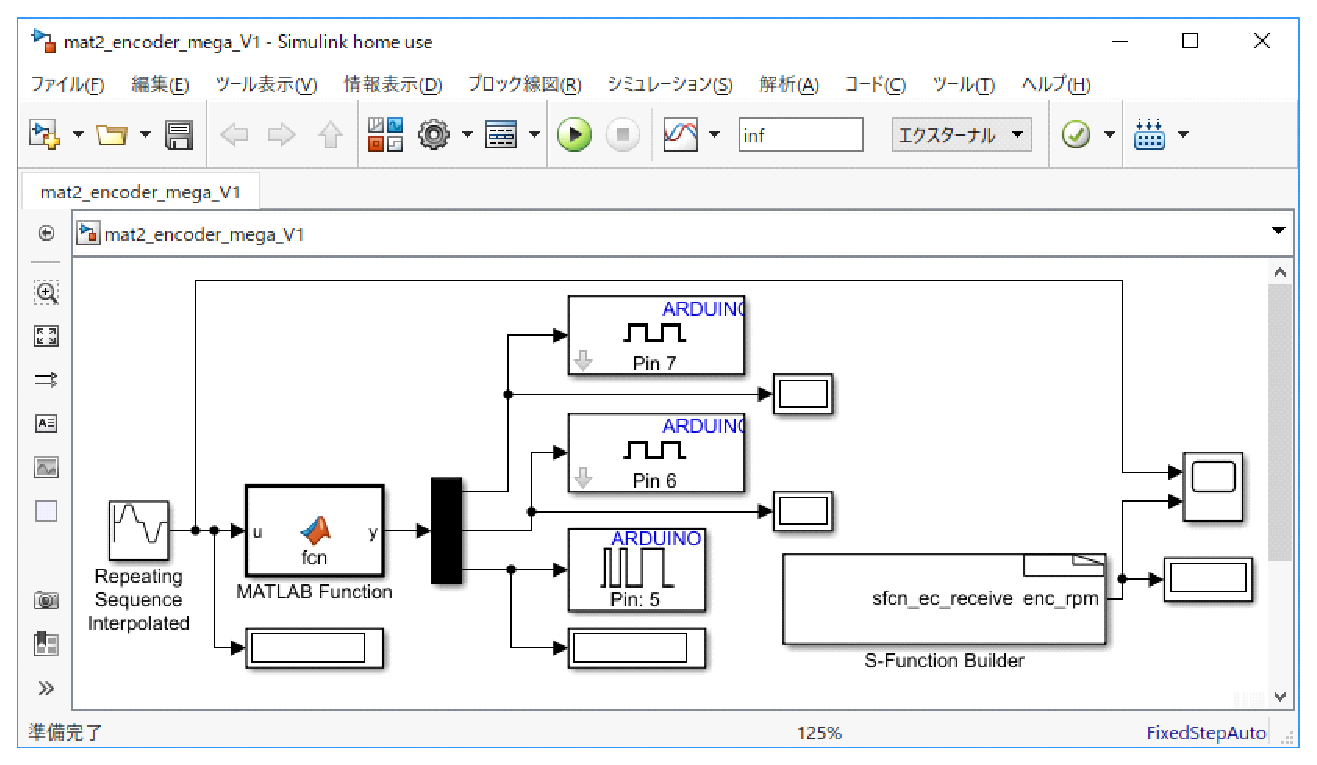
\includegraphics[width=380pt]{fig/fig303.eps}
    \caption{Matlab/Simulinkモデル}
    \label{fig303}
\end{figure}

\begin{figure}[htbp]
    \centering
    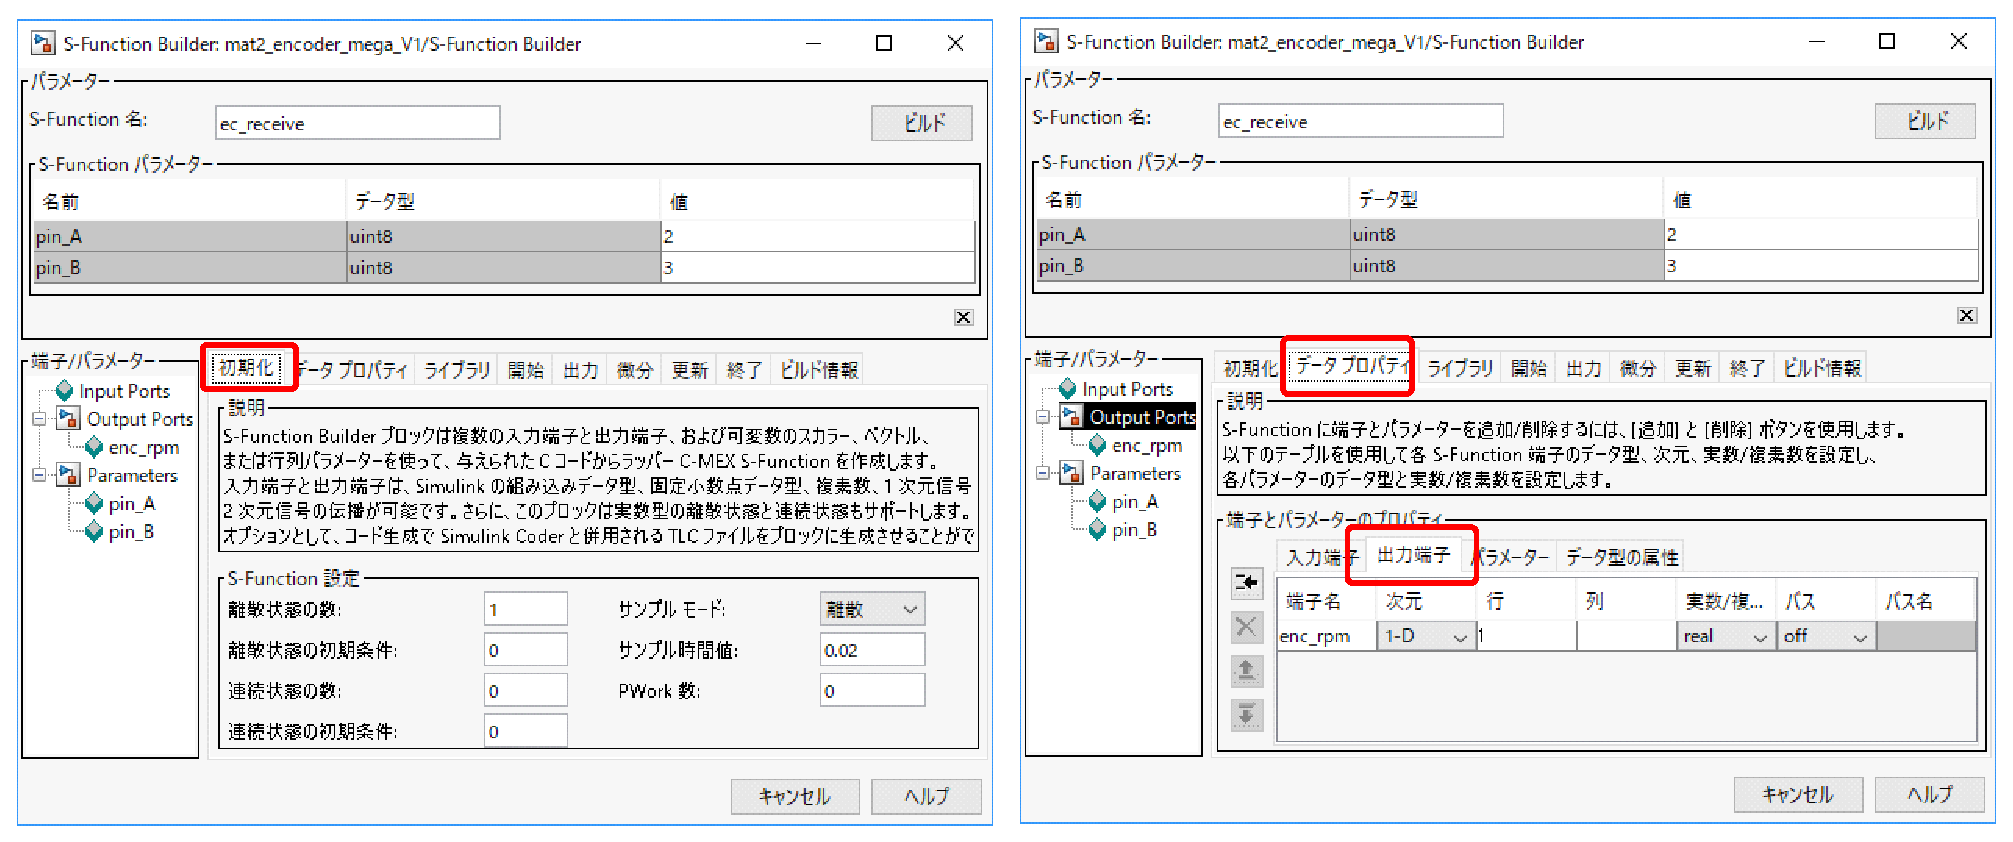
\includegraphics[width=380pt]{fig/fig304.eps}
    \caption{S-Function Builder}
    \label{fig304}
\end{figure}

\begin{figure}[htbp]
    \centering
    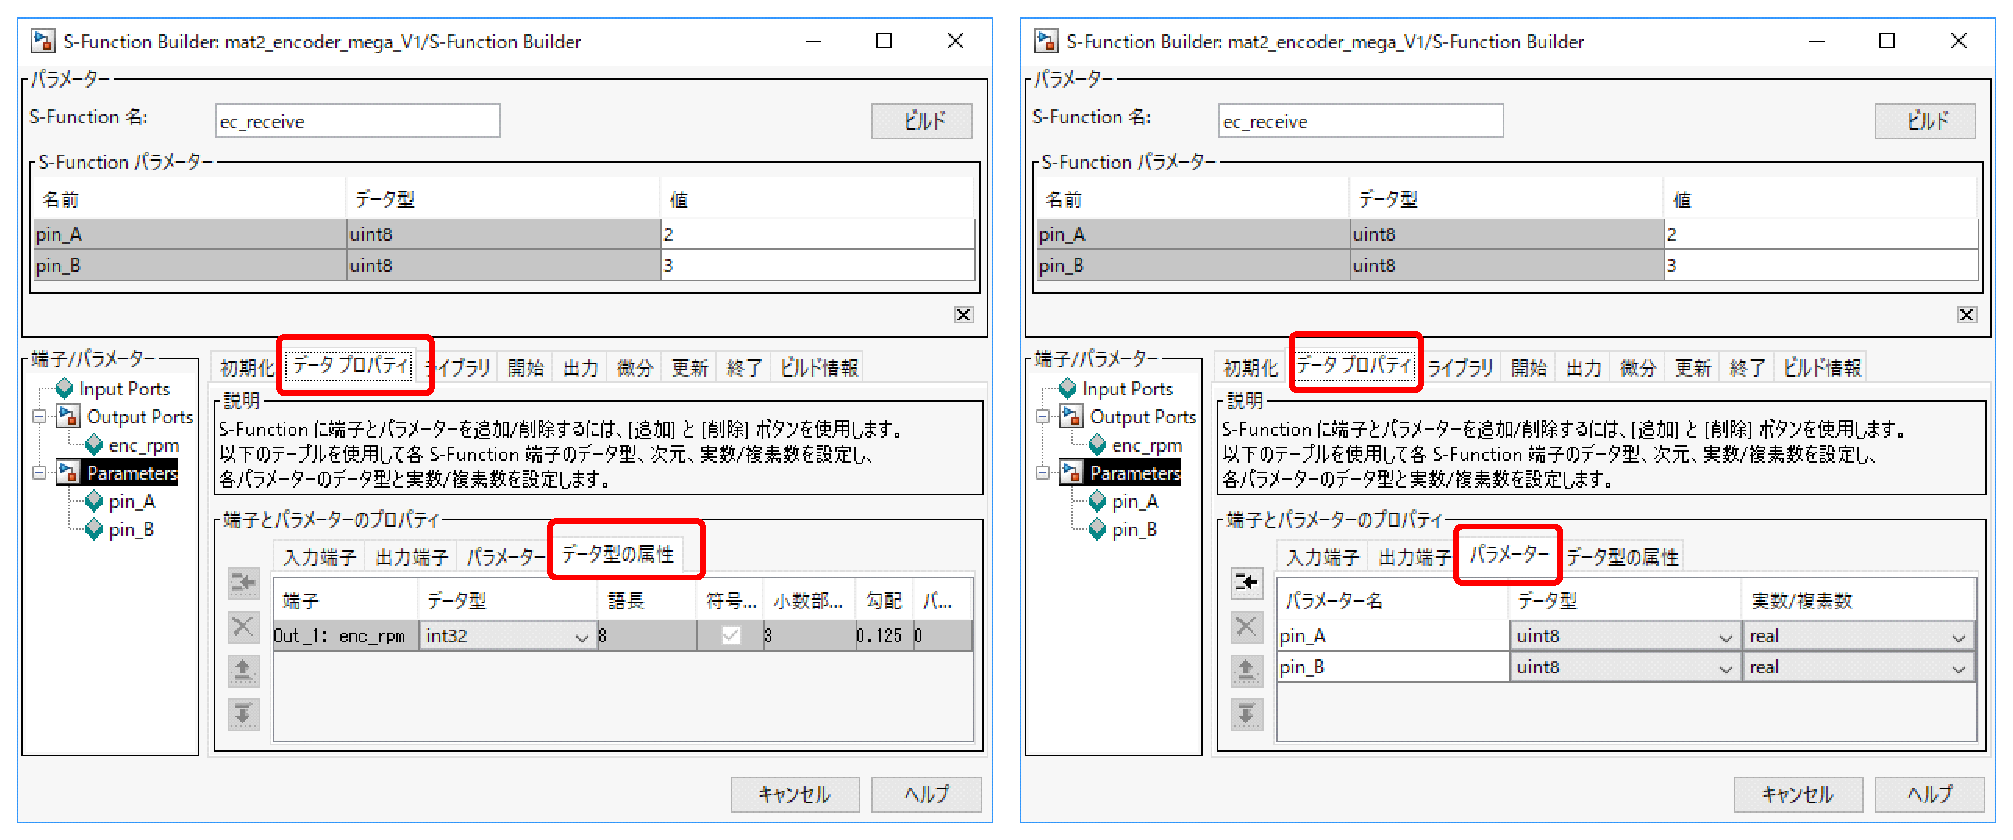
\includegraphics[width=380pt]{fig/fig305.eps}
    \caption{S-Function Builder}
    \label{fig305}
\end{figure}

\begin{figure}[htbp]
    \centering
    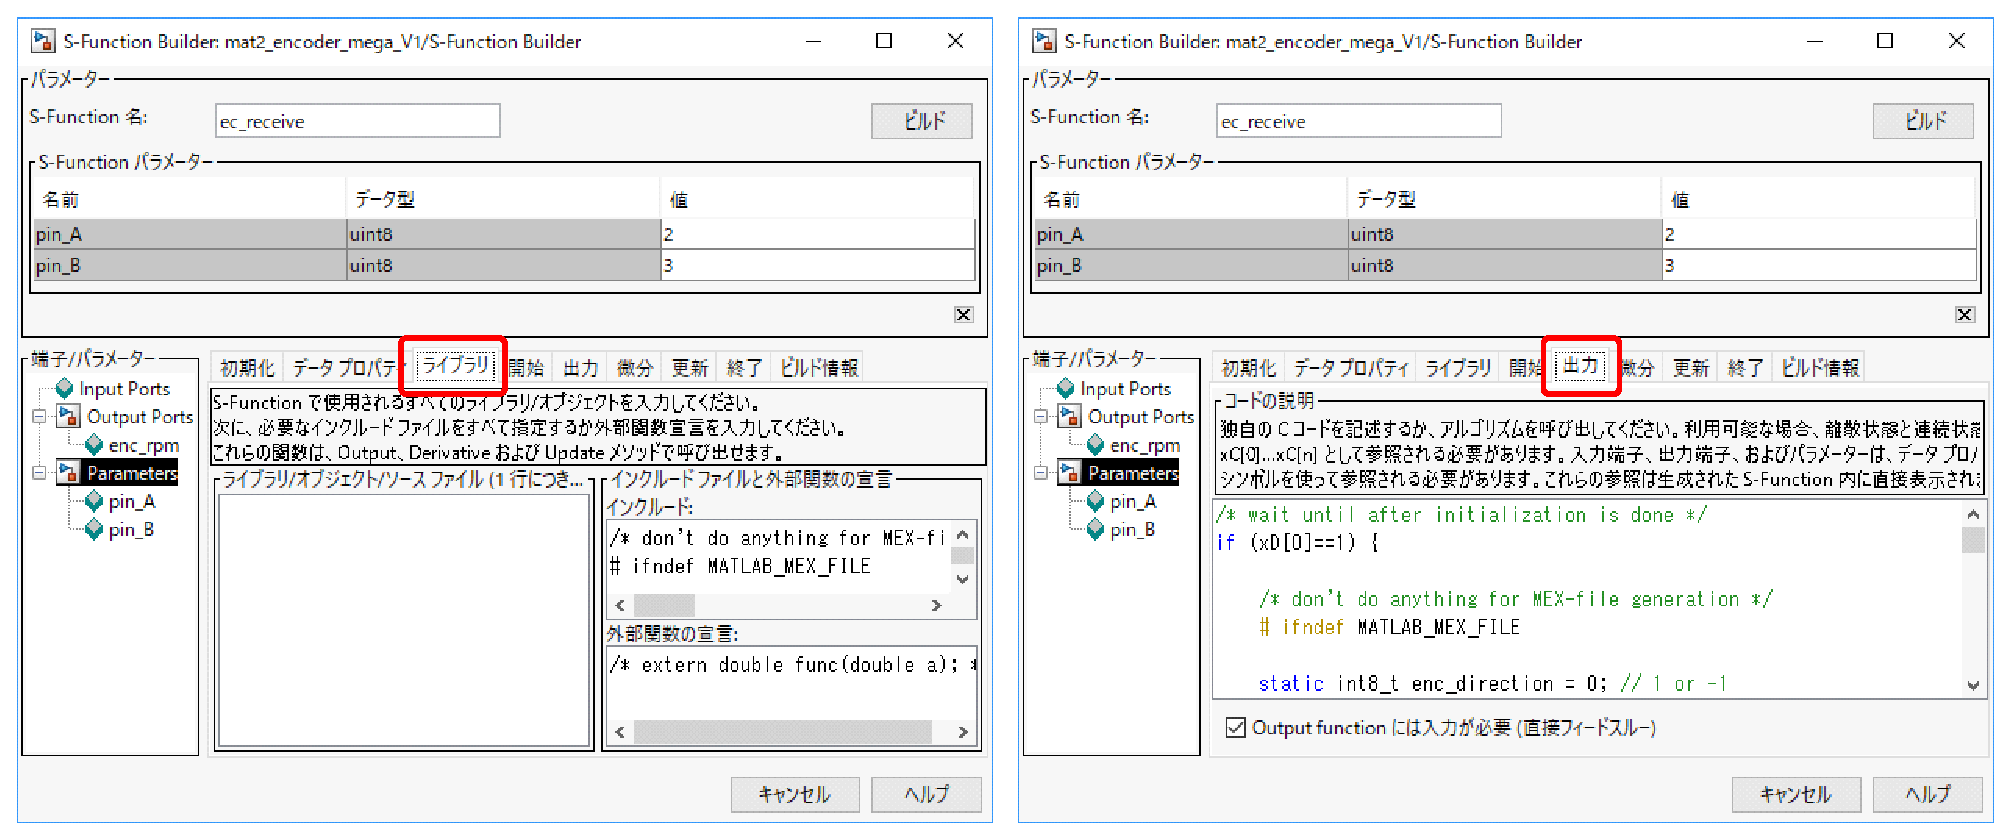
\includegraphics[width=380pt]{fig/fig306.eps}
    \caption{S-Function Builder}
    \label{fig306}
\end{figure}

\begin{figure}[htbp]
    \centering
    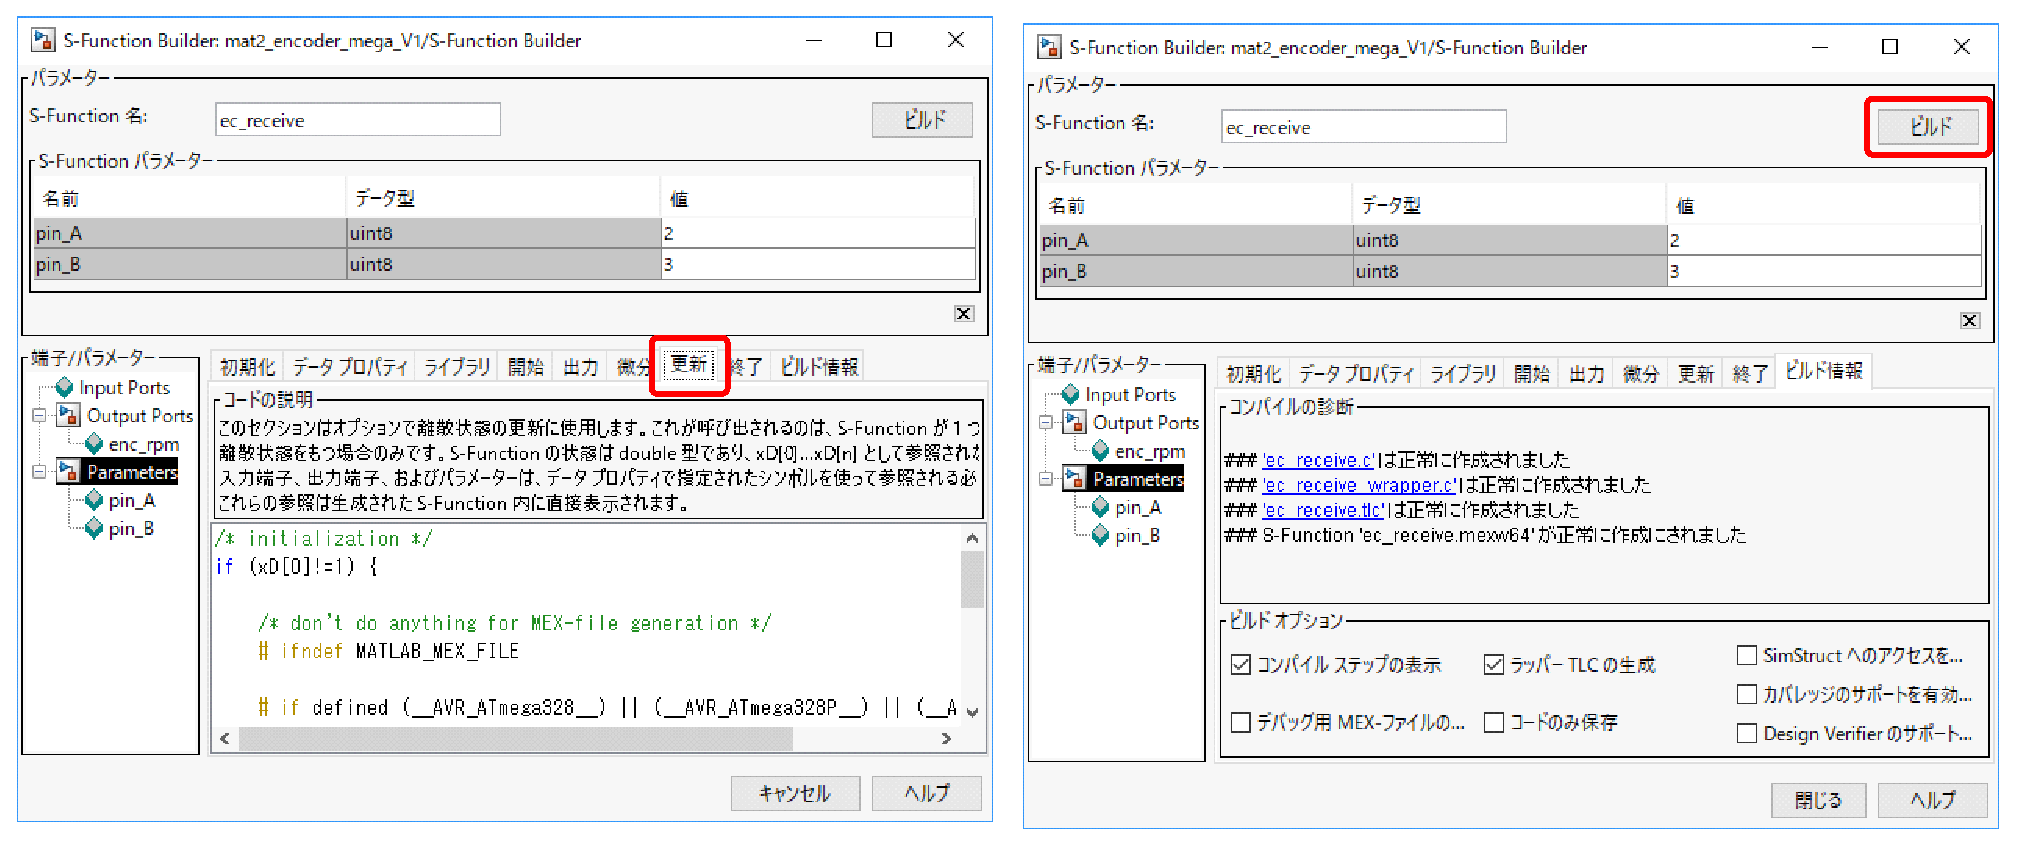
\includegraphics[width=380pt]{fig/fig307.eps}
    \caption{S-Function Builder}
    \label{fig307}
\end{figure}   

\begin{figure}[htbp]
    \centering
    \includegraphics[width=300pt]{fig/fig308.eps}
    \caption{S-Function Builder ライブラリ インクルード}
    \label{fig308}
\end{figure}   

\begin{figure}[htbp]
    \centering
    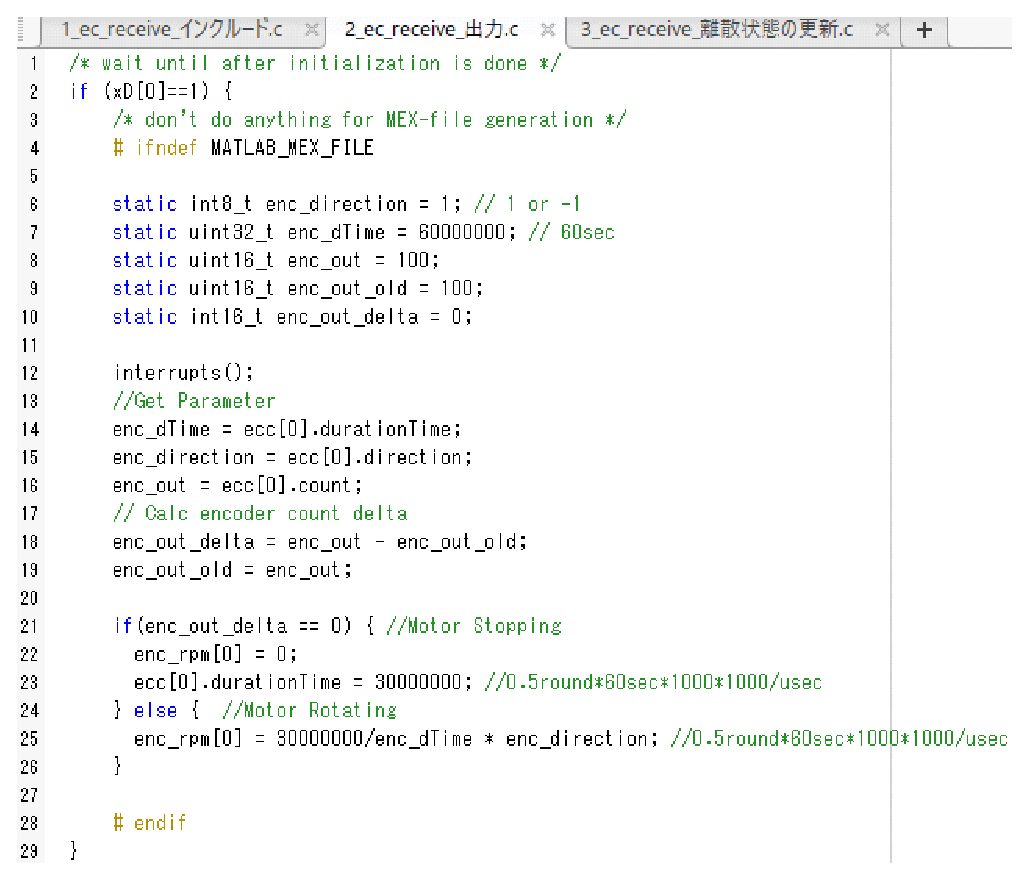
\includegraphics[width=320pt]{fig/fig309.eps}
    \caption{S-Function Builder 出力}
    \label{fig309}
\end{figure}  

\begin{figure}[htbp]
    \centering
    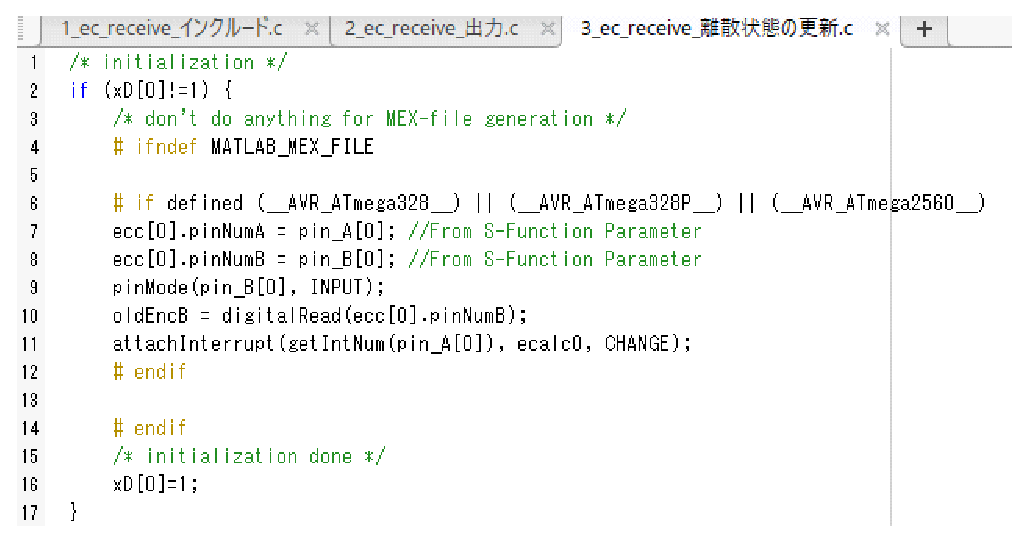
\includegraphics[width=320pt]{fig/fig310.eps}
    \caption{S-Function Builder 離散状態の更新}
    \label{fig310}
\end{figure}  


\clearpage
\section{実行}\label{ux811aux69cbux6210}

Scopeブロックのグラフ表示を立ち上げた状態で "実行" することで、
回転数測定結果をリアルタイムにグラフを描写できます。
実行例としてFig.\ref{fig311}に示します。
操作量に応じて、回転数が高くなることが確認できます。
\begin{figure}[htbp]
    \centering
    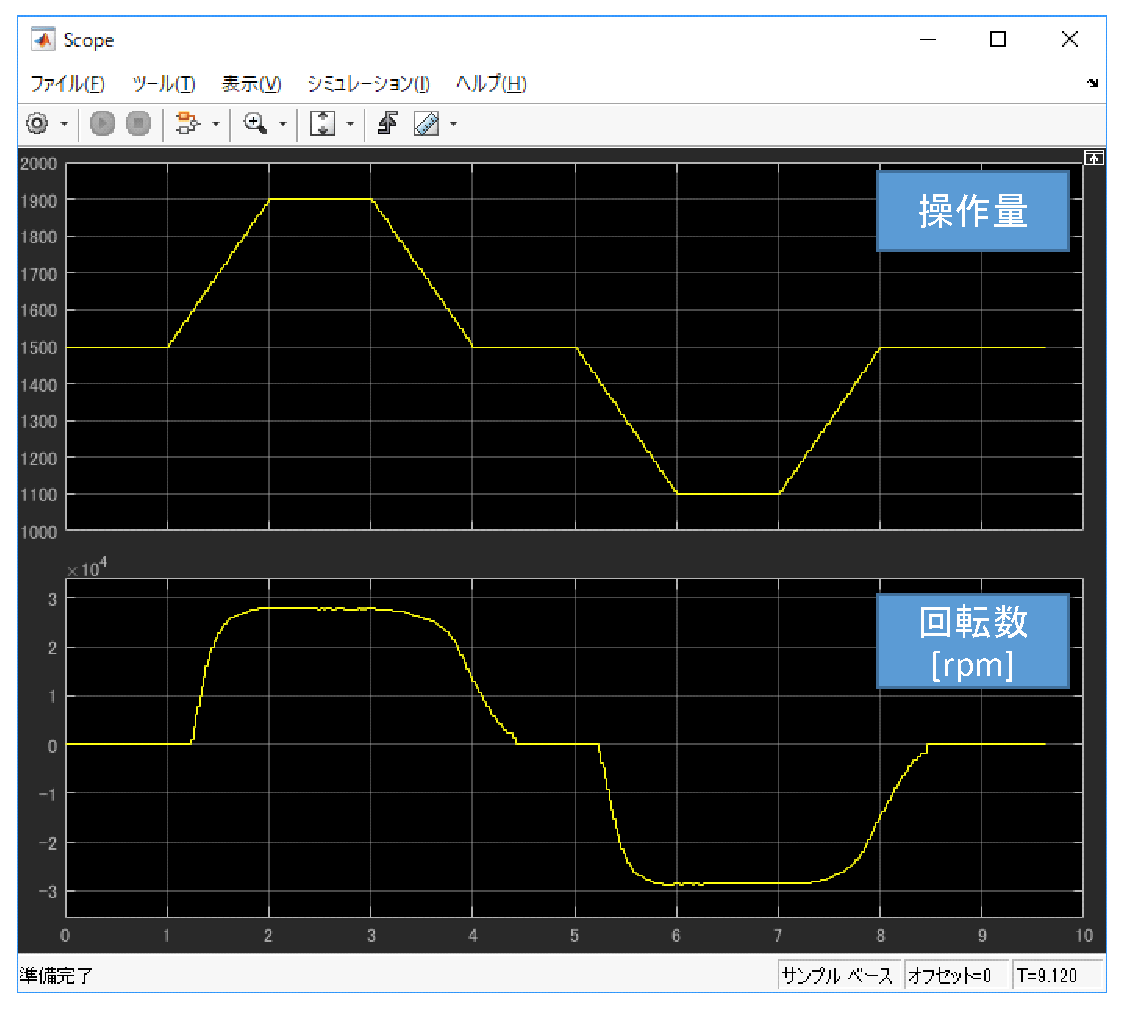
\includegraphics[width=200pt]{fig/fig311.eps}
    \caption{回転数の計測結果}
    \label{fig311}
\end{figure}

正しく回転数が計測できているか確認する方法として、
次のような外部計測器(Fig.\ref{fig312})を使う方法があります。
例えば回転計を使用する場合は、エンコーダの円盤に反射シールを張り付け、
モータを定常回転させれば回転数を計測できます。

\begin{itemize}
    \tightlist
    \item
    回転計:非接触デジタルタコメーター DT2234B
    \item
    オシロスコープ:MiniDSO DS203
    \end{itemize}

\begin{figure}[htbp]
    \centering
    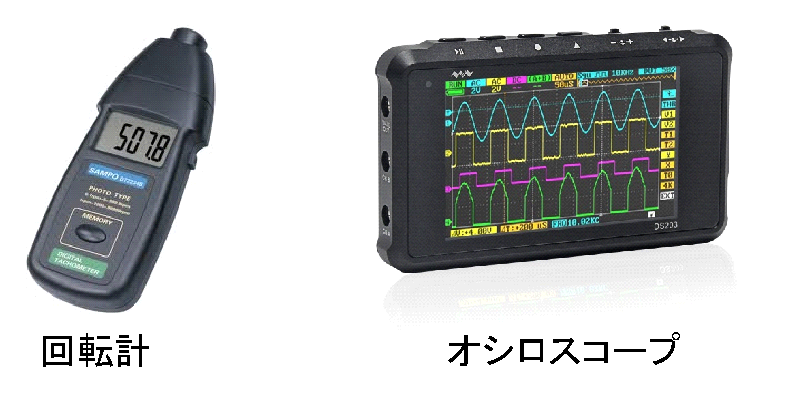
\includegraphics[width=200pt]{fig/fig312.eps}
    \caption{計測器}
    \label{fig312}
\end{figure}

\chapter{Matlab/SimulinkとArduinoでモータ回転数制御をしよう}
\thispagestyle{fancy}
\section{ハード構成}\label{ux5168ux4f53ux69cbux6211}

ハード構成、および電気回路は第3章と同じで、Fig.\ref{fig401}になります。

\begin{figure}[htbp]
    \centering
    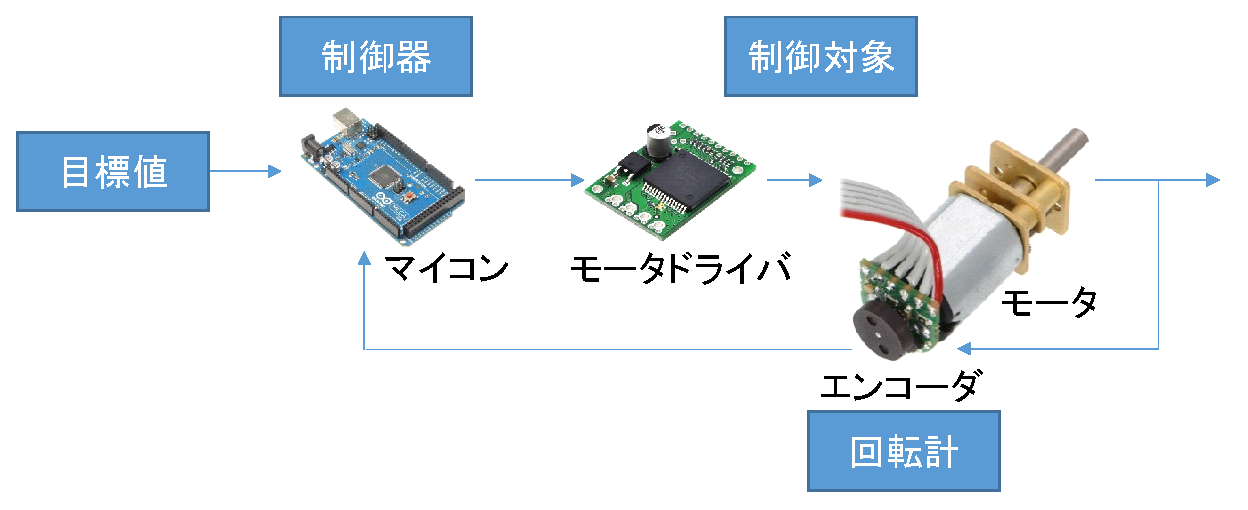
\includegraphics[width=300pt]{fig/fig401.eps}
    \caption{ハード構成}
    \label{fig401}
\end{figure}


\section{PID制御モデル}\label{ux6a5fux4f53ux306eux72b6ux614bux3068ux30b5ux30a4ux30ba}

SimulinkによるPID制御モデルはFig.\ref{fig402}の通りです。
PID Controller ブロックのパラメータはFig.\ref{fig403}の値を入力しました。
Saturation ブロックのパラメータはFig.\ref{fig404}の値を入力しました。
今回のモータはDC6Vで29000~30000rpmにて回るので、
Saturation1 ブロックにはモータ最大回転数より若干低い値を入力します。
Saturation2 ブロックには操作量の上下限で飽和するようにします。

\begin{figure}[htbp]
    \centering
    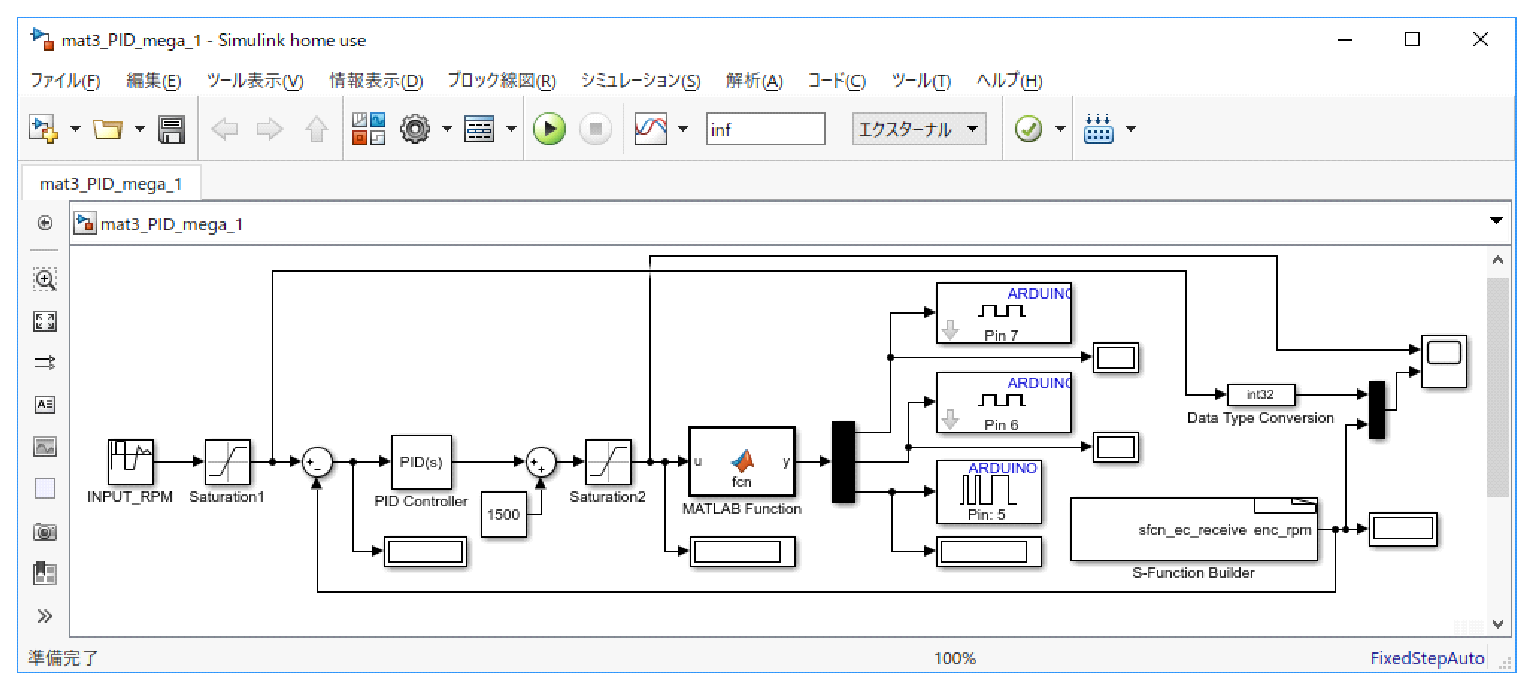
\includegraphics[width=389pt]{fig/fig402.eps}
    \caption{PID制御のSimulinkモデル}
    \label{fig402}
\end{figure}

\begin{figure}[htbp]
    \centering
    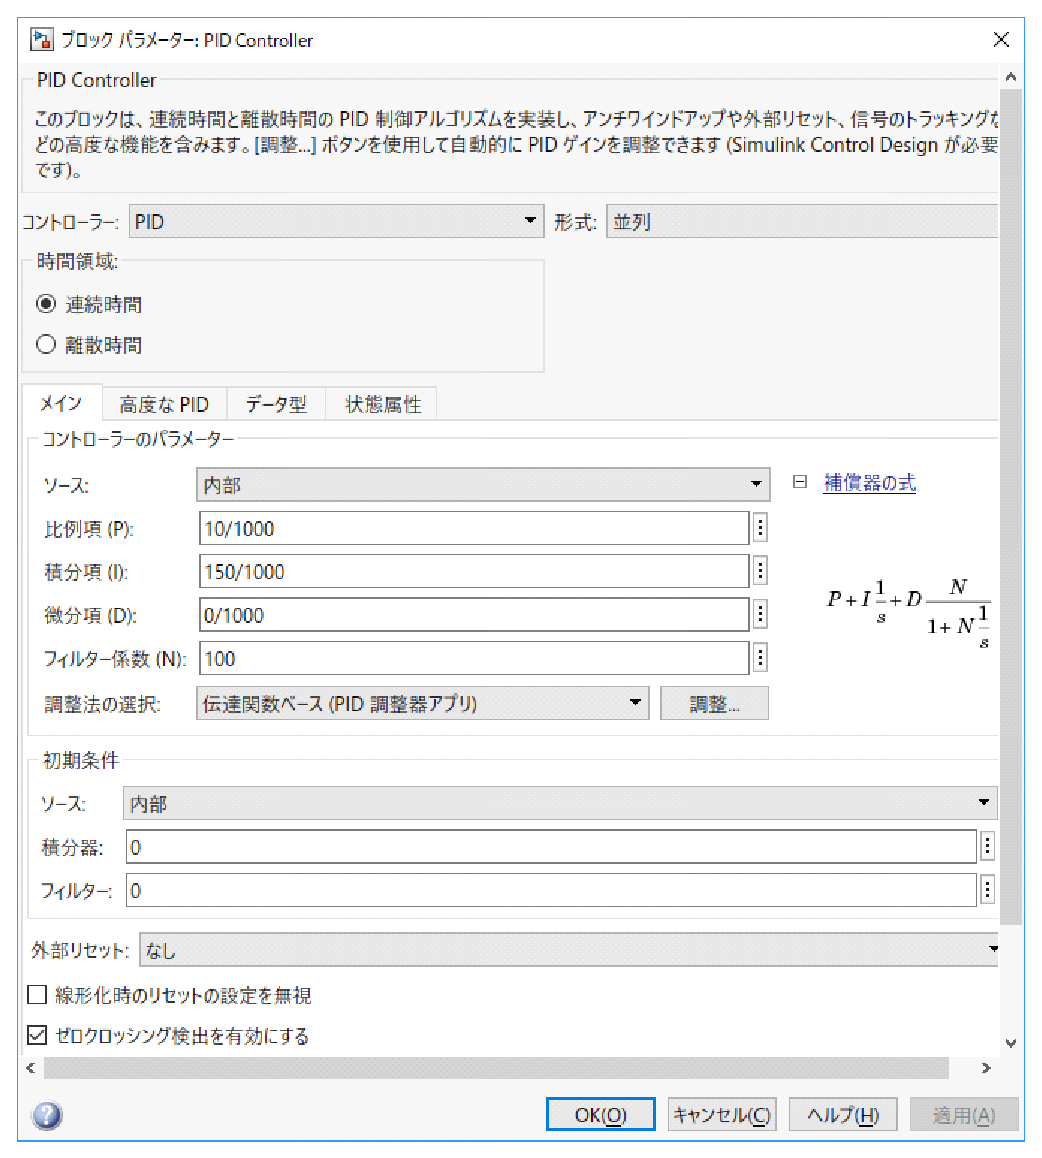
\includegraphics[width=250pt]{fig/fig403.eps}
    \caption{PID Controller ブロック パラメータ}
    \label{fig403}
\end{figure}

\begin{figure}[htbp]
    \centering
    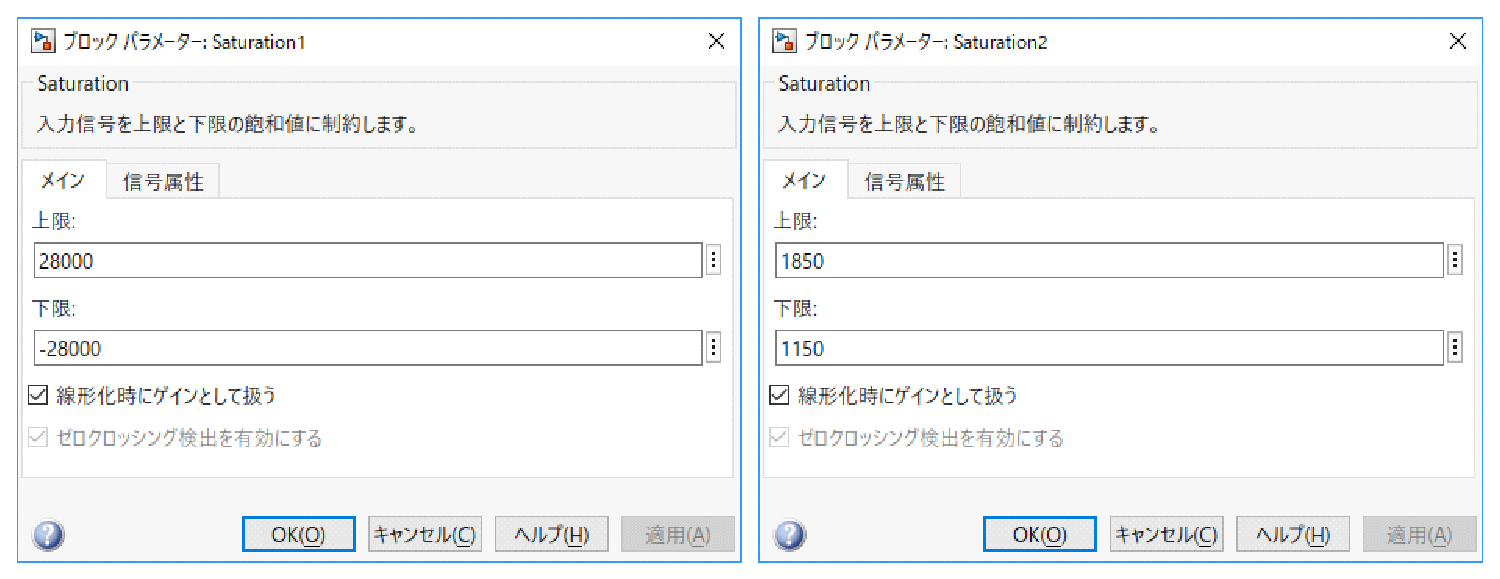
\includegraphics[width=350pt]{fig/fig404.eps}
    \caption{Saturation ブロック パラメータ}
    \label{fig404}
\end{figure}


%\clearpage
\section{実行}\label{ux30a2ux30fcux30e0ux69cbux6210ux306eux8a73ux7d30}

回転数の計測結果をFig.\ref{fig405}に示します。
回転数の黄色線が目標の回転数で、青線が実測値になります。
目標に対して実測値がおおむね追従していることが確認できます。

\begin{figure}[htbp]
    \centering
    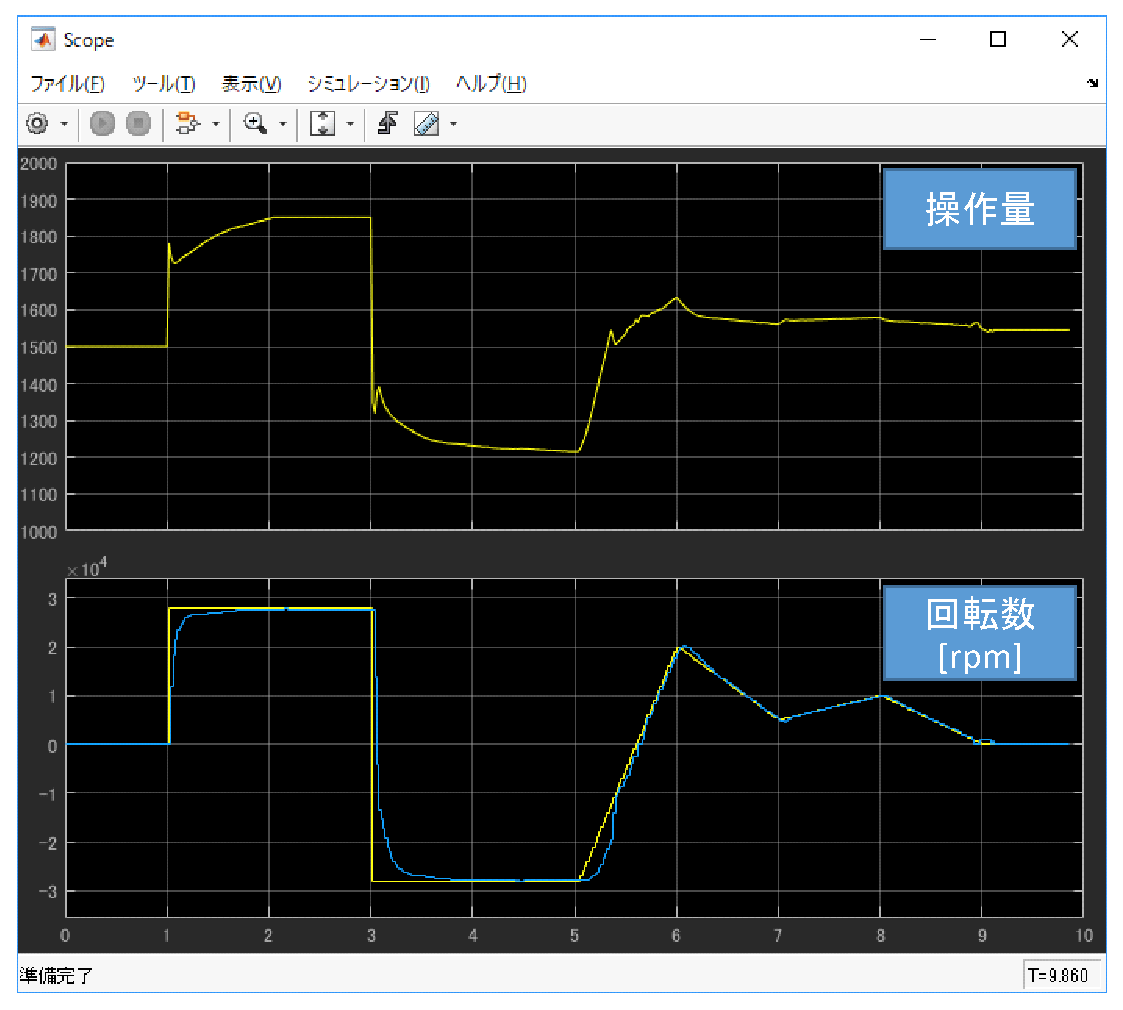
\includegraphics[width=200pt]{fig/fig405.eps}
    \caption{回転数の計測結果}
    \label{fig405}
\end{figure}


\section{ロボットへの実装例}\label{ux7a4dux5c64ux65b9ux5411ux306eux5272ux308cux9632ux6b62ux69cbux6210}

Fig.\ref{fig101}に示したロボットへの実装例になります。
本ロボットは脚ユニットを4脚使用しています。
そのハード構成はFig.\ref{fig406}の通りです。
中央制御基板で受信機からのラジコン信号を読み取り、
I2C通信で各脚制御基板に回転数目標値を出力しています。

Fig.\ref{fig407}に中央制御基板のSimulinkモデルを示します。
ラジコン信号の読み取り方法は
Using an RC Controller with Arduino and Simulink\cite{MathWors_RC_receive}
を参考にしました。
読み取ったラジコン信号のバルス幅をローパスフィルタにかけ、
パルス幅から回転数目標に変換し、
I2Cブロックに入力するため、回転数目標値を+-の符号を含め3byteのデータに変換しています。

Fig.\ref{fig408}に脚制御基板のSimulinkモデルを示します。
I2C通信をS-function ブロックで実現する方法は
ADLX345 i2c Driver for Arduino Mega\cite{MathWors_I2C}
を参考にしました。
I2C Masterから読み取った回転数目標値は、3byteデータを復号して
Fig.\ref{fig402}で作製したモデルの入力側に接続しています。

実行例をFig.\ref{fig409}に示します。
手で操作したプロポの挙動に応じて、回転数を制御することができます。

\begin{figure}[htbp]
    \centering
    \includegraphics[width=350pt]{fig/fig406.eps}
    \caption{ロボットへの実装}
    \label{fig406}
\end{figure}

\begin{figure}[htbp]
    \centering
    \includegraphics[width=389pt]{fig/fig407.eps}
    \caption{中央制御基板のSimulinkモデル (I2C Master)}
    \label{fig407}
\end{figure}

\begin{figure}[htbp]
    \centering
    \includegraphics[width=389pt]{fig/fig408.eps}
    \caption{脚制御基板のSimulinkモデル (I2C Slave)}
    \label{fig408}
\end{figure}

\begin{figure}[htbp]
    \centering
    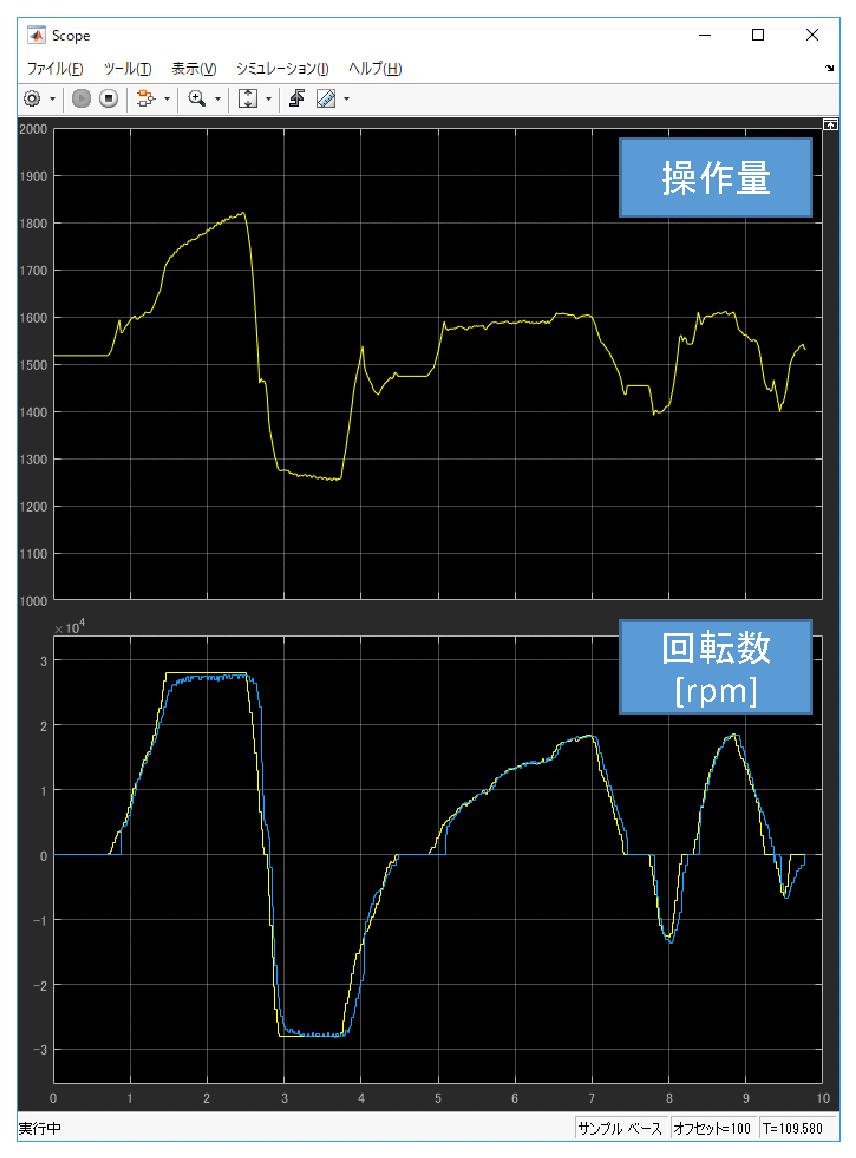
\includegraphics[width=200pt]{fig/fig409.eps}
    \caption{実行例}
    \label{fig409}
\end{figure}



%------------------------------------------------------------------
%参考文献
\begin{thebibliography}{20}
\bibitem{kawasaki_public_HP}かわさきロボット競技大会 公式HP\\
  \url{http://www.kawasaki-net.ne.jp/robo/}
\bibitem{MathWorks_HP}MathWorks ストア\\
  \url{https://jp.mathworks.com/store/link/products/}
\bibitem{Simulink_examples}Simulink Support Package for Arduino Hardware Examples\\
  \url{http://jp.mathworks.com/help/supportpkg/arduino/examples.html}
\bibitem{Win_SDK1}Windows SDK 7.1のインストール時のはまりポイント\\
  \url{http://d.hatena.ne.jp/kfujieda/20140827/1409137229}
\bibitem{Win_SDK2}How can I install sdk 7.1 on windows 10 ???\\
  \url{https://jp.mathworks.com/matlabcentral/answers/}\\
    233850-how-can-i-install-sdk-7-1-on-windows-10/
\bibitem{switch-science_HP}スイッチサイエンス\\
  \url{https://www.switch-science.com/}
\bibitem{pololu_HP_driver}Pololu HP モータドライバ VNH5019\\
  \url{https://www.pololu.com/product/1451}
\bibitem{pololu_HP_encoder}Pololu HP 磁気式エンコーダ\\
  \url{https://www.pololu.com/product/3081}
\bibitem{wiki_PID}ウィキペディア PID制御\\
  \url{https://ja.wikipedia.org/wiki/PID制御}
\bibitem{MathWors_RC_receive}Using an RC Controller with Arduino and Simulink\\
  \url{https://jp.mathworks.com/videos/}\\
    using-an-rc-controller-with-arduino-and-simulink-91738.html
\bibitem{MathWors_I2C}ADLX345 i2c Driver for Arduino Mega\\
  \url{https://jp.mathworks.com/matlabcentral/}\\
    fileexchange/41027-adlx345-i2c-driver-for-arduino-mega/
\end{thebibliography}
\thispagestyle{empty}  
%------------------------------------------------------------------
%\appendix % 付録

%------------------------------------------------------------------
\backmatter % 後書きの開始
\chapter{奥付}
\thispagestyle{empty} 

\section*{発行}
でし・ぷろんぷと \\
2018年8月10日 初版第1刷発行

\section*{著者}
santny

\section*{フォロー}
takarakasai \\
kyo46

\section*{印刷}
製本直送.com

\section*{Web} 
http://deshi-prompt.github.io/

\section*{Mail}
ada.robo1@gmail.com


%\newpage 
%\pagestyle{empty}
%\printindex
%
%
\end{document}